% Official MDPI/Sustainability template class; downloaded 2026-09-04.
\documentclass[sustainability,article,submit,moreauthors]{Definitions/mdpi}
\firstpage{1}
\makeatletter
\setcounter{page}{\@firstpage}
\makeatother
\pubvolume{1}
\issuenum{1}
\articlenumber{0}
\pubyear{2026}
\copyrightyear{2026}
\datereceived{}
\daterevised{}
\dateaccepted{}
\datepublished{}

\usepackage{bm}
\usepackage{mathtools}
\usepackage{placeins}
\usepackage{threeparttable}
\numberwithin{equation}{section}
\setlength{\headheight}{25pt}
\newcommand{\sym}[1]{\ifmmode^{#1}\else\(^{#1}\)\fi}

\Title{Agricultural Total Factor Productivity and High-Quality Economic Development in China: Regional Disparities, Coupling Coordination, and Spatial Dynamics}
\newcommand{\orcidauthorA}{0009-0005-7353-9159}
\Author{Pengpeng Zhou $^{1}$\orcidA{}, Yile Wang $^{1}$*}
\AuthorNames{Pengpeng Zhou and Yile Wang}
\address{$^{1}$ \quad Beijing Technology and Business University; e-mail: m3126211047@163.com (P.Z.); wyl13393401611@126.com (Y.W.)}
\corres{Correspondence: wyl13393401611@126.com (Y.W.)}

\abstract{This study examines whether, through which channels, and under what development conditions agricultural total factor productivity (Agricultural TFP) is associated with high-quality economic development across 31 provincial-level regions in China during 2016--2020. High-quality development is measured with a 16-indicator composite index covering economic performance, government governance, urban--rural coordination, green development, and shared welfare. Agricultural TFP is measured with an output-oriented DEA--Malmquist index; because the index measures growth rather than an absolute level, 2016 is used as a common base of 1.000 and subsequent values are chained products. The empirical design combines kernel-density estimates, Dagum Gini decomposition, global and local Moran's $I$, a coupling-coordination model, two-way fixed effects, a spatial Durbin model, a panel threshold model, and a spatial Markov chain. The high-quality development mean increased from 0.365 to 0.462 and its Dagum Gini coefficient fell from 0.215 to 0.141. Cumulative Agricultural TFP increased from 1.000 to 1.386, while its interprovincial dispersion widened. The two systems remained highly coupled in relative terms ($C=0.900$--$0.969$), and the mean coordination degree rose from 0.499 to 0.662, mainly as their joint development level increased. High-quality development displayed significant positive global spatial autocorrelation in every year; cumulative TFP became significant from 2018 onward. The preferred two-way fixed-effects elasticity is 0.446 ($p=0.029$). Spatial impacts show a significant direct effect of 0.368 ($p<0.001$) and total effect of 0.665 ($p=0.004$), but an imprecise indirect effect of 0.297 ($p=0.164$). A threshold is detected at log GDP per capita 11.069: the TFP elasticity is 0.375 ($p=0.036$) below the threshold and $-0.344$ ($p=0.133$) above it. Markov transitions are strongly persistent, whereas differences across neighborhood conditions are only marginally significant ($p=0.087$). The evidence therefore supports a cautious interpretation: Agricultural TFP is positively associated with local development quality, especially at lower development stages, but a stable cross-provincial spillover and a causal threshold are not established.}
\keyword{Agricultural Total Factor Productivity; high-quality economic development; coupling coordination degree; spatial autocorrelation; spatial Durbin model; spatial Markov chain}

\begin{document}

\section{Introduction}

China's agricultural transformation is increasingly evaluated not only by output growth but also by the efficiency with which land-related inputs, machinery, energy, and intermediate inputs are converted into output. Total factor productivity (TFP) summarizes the part of output performance not explained by measured input accumulation \cite{liu1999}. Agricultural TFP can therefore capture technological progress and efficiency change, but it does not automatically imply broader improvements in income distribution, public services, environmental quality, or urban--rural coordination. High-quality economic development is multidimensional, so the translation from productivity gains to development quality must be tested rather than assumed.

This question is particularly relevant in China after the policy emphasis on high-quality development was formalized in 2017. The institutional shift may have increased attention to efficiency, structural transformation, and balanced development, but it does not mean that TFP was newly created in that year or that subsequent changes can be attributed to the policy milestone without identification. The relevant empirical issue is whether productivity growth is associated with development quality, whether the association differs across regions and development stages, and whether it is organized spatially.

The existing evidence leaves several issues open. Solow-residual studies require restrictive assumptions about competition, returns to scale, and factor-income shares, while stochastic-frontier models require distributional and functional-form choices. Moreover, studies often examine productivity, development quality, regional inequality, or spatial dependence separately. Less is known about how cumulative agricultural productivity growth and a multidimensional quality index evolve together in a short provincial panel, whether their distributions converge, and whether an observed association reflects local effects, cross-provincial transmission, development-stage heterogeneity, or persistent spatial states.

This paper addresses these gaps using a balanced panel of 31 provincial-level regions from 2016 to 2020. We construct the high-quality development index from 16 indicators using entropy-based variation and Spearman-correlation conflict information, and measure cumulative Agricultural TFP with an output-oriented DEA--Malmquist index. We then combine distributional and spatial tools with econometric tests. The analysis asks four questions: (i) how did the two indicators evolve and how did their regional disparities change; (ii) did the two systems become more closely coordinated; (iii) are their spatial associations and local clusters statistically detectable; and (iv) does the Agricultural TFP association vary with development stage, operate through neighboring provinces, or persist across spatially conditioned states?

The study makes three contributions. First, it places cumulative productivity growth and multidimensional development quality in a common measurement framework while making the common TFP base-year implication explicit. Second, it connects kernel density, Dagum decomposition, Moran statistics, coupling coordination, fixed-effects regressions, spatial impacts, threshold regimes, and Markov transitions in a single empirical sequence. Third, it separates evidence that is robust across specifications from evidence that is exploratory in this short panel. The main results are that development quality rises and converges, cumulative TFP rises but becomes more dispersed, and the two systems remain highly coupled in relative terms while their coordination improves with the joint level of development. The fixed-effects association is positive, the spatial direct effect is significant but the indirect effect is imprecise, the association is concentrated below an income threshold, and development states are persistent. These findings motivate the hypotheses below and guide the cautious interpretation of the subsequent results.

\section{Literature and hypotheses}

Nonparametric productivity measurement decomposes productivity change into movements toward the production frontier and shifts in the frontier itself \cite{fare1994}. Applications to Chinese agriculture emphasize that productivity growth can differ markedly across regions because input structures, technology adoption, and resource constraints vary \cite{fan2002}. Productivity gains may support high-quality development through at least three channels: higher real income and fiscal capacity, the release and reallocation of labor, and lower resource intensity per unit of output. Yet these mechanisms depend on local institutions, market access, public services, and environmental governance.

International comparisons of Chinese agricultural productivity likewise
distinguish technical efficiency from technical progress \cite{che2010}.
This distinction motivates measuring productivity changes separately from
the accumulation of observed inputs.

Spatial dependence is also plausible. Adjacent provinces share infrastructure, ecological conditions, factor markets, and technology-diffusion networks. Local indicators of spatial association can reveal whether high- and low-value areas form statistically significant clusters \cite{moran1950,anselin1995}. A spatial Durbin specification further separates own-region responses from feedback-adjusted effects transmitted through neighbors \cite{lesage2009}.

Finally, the return to Agricultural TFP may vary with development stage. In lower-income provinces, agricultural productivity can relax binding resource and income constraints. At higher income levels, innovation, services, environmental governance, and human capital may become relatively more important. Panel threshold methods offer a direct way to evaluate this possibility \cite{hansen1999}. Spatial Markov methods additionally distinguish persistence from neighborhood-conditioned mobility. These arguments motivate the following hypotheses:

\begin{enumerate}[label=H\arabic*.,leftmargin=2.4em]
\item Agricultural TFP is positively associated with high-quality economic development.
\item High-quality economic development and Agricultural TFP exhibit positive spatial dependence.
\item Agricultural TFP generates positive direct effects, while indirect spillovers depend on regional transmission channels.
\item The Agricultural TFP coefficient changes with the level of economic development.
\item High-quality development states are persistent, and neighborhood conditions may alter transition probabilities.
\end{enumerate}

\section{Materials and Methods}

\subsection{Sample and variables}

The balanced panel contains 155 province--year observations: 31 provincial-level regions observed annually from 2016 to 2020. Hong Kong, Macao, and Taiwan are excluded because comparable input and outcome series are unavailable. The underlying indicators were assembled from the China Statistical Yearbook and China Rural Statistical Yearbook and then consolidated into the project's analysis dataset. The eastern, central, and western groupings contain 11, 8, and 12 provinces, respectively.

The outcome is the high-quality economic development index, denoted by $Y_{it}$. The core explanatory variable is cumulative Agricultural TFP, denoted by $TFP_{it}$. The baseline regressions include log population density and the share of the primary sector as controls. GDP per capita is used as the threshold variable.

\begin{table}[H]
\centering
\caption{Indicator system for high-quality economic development}
\label{tab:indicator}
\small
\begin{tabularx}{\textwidth}{p{3.4cm} X c}
\toprule
Dimension & Secondary indicator & Direction \\
\midrule
\multirow{4}{3.4cm}{Economic performance quality}
& GDP per capita (PCGDP) & $+$ \\
& Retail sales of consumer goods per capita (PCRS) & $+$ \\
& Growth rate of tertiary-industry value added (TIG) & $+$ \\
& Share of high-technology operating income (HBTP) & $+$ \\
\addlinespace
\multirow{2}{3.4cm}{Government economic governance}
& Fiscal self-sufficiency rate (FSG) & $+$ \\
& Government consumption rate (GCR) & $+$ \\
\addlinespace
\multirow{4}{3.4cm}{Urban--rural coordination}
& Resident-population urbanization rate (IPR) & $+$ \\
& Urban--rural income ratio (RUUR) & $-$ \\
& Urban road area per capita (PCURA) & $+$ \\
& Public transport vehicles per 10,000 residents (PTVP) & $+$ \\
\addlinespace
\multirow{3}{3.4cm}{Green and low-carbon development}
& Energy consumption per unit of GDP (WEI) & $-$ \\
& Pollutant emissions per unit of GDP (SDEI) & $-$ \\
& Electricity-consumption elasticity coefficient (EPES) & $-$ \\
\addlinespace
\multirow{3}{3.4cm}{Shared development and welfare}
& Fiscal health expenditure per capita (HESP) & $+$ \\
& Urban gas coverage (UGPR) & $+$ \\
& Urban water coverage (UWPR) & $+$ \\
\bottomrule
\end{tabularx}
\end{table}

\subsection{Construction of the high-quality development index}
For a positive indicator, min--max normalization is defined as
\begin{equation}
z_{ij}^{+}=\frac{x_{ij}-\min_i x_{ij}}{\max_i x_{ij}-\min_i x_{ij}}.
\label{eq:positive}
\end{equation}
For a negative indicator, the direction is reversed:
\begin{equation}
z_{ij}^{-}=\frac{\max_i x_{ij}-x_{ij}}{\max_i x_{ij}-\min_i x_{ij}}.
\label{eq:negative}
\end{equation}
The normalized share of observation $i$ in indicator $j$ is
\begin{equation}
p_{ij}=\frac{z_{ij}}{\sum_{i=1}^{n}z_{ij}}.
\label{eq:share}
\end{equation}
Entropy and the associated variation coefficient are
\begin{equation}
e_j=-\frac{1}{\ln n}\sum_{i=1}^{n}p_{ij}\ln p_{ij}.
\label{eq:entropy}
\end{equation}
\begin{equation}
d_j=1-e_j.
\label{eq:variation}
\end{equation}
To reduce sensitivity to nonlinear monotonic dependence, conflict is calculated using the absolute Spearman correlation $\rho_{jk}^{S}$:
\begin{equation}
\delta_j=\sum_{k=1}^{m}\left(1-\left|\rho_{jk}^{S}\right|\right).
\label{eq:conflict}
\end{equation}
The information content and normalized weight are
\begin{equation}
C_j=d_j\delta_j.
\label{eq:information}
\end{equation}
\begin{equation}
w_j=\frac{C_j}{\sum_{j=1}^{m}C_j}.
\label{eq:weight}
\end{equation}
The composite score is therefore
\begin{equation}
Y_i=\sum_{j=1}^{m}w_j z_{ij}.
\label{eq:hqd}
\end{equation}

Based on the above formula, we can calculate the value of y. The following is the three-dimensional surface plot of y.

\begin{figure}[H]
	\centering
	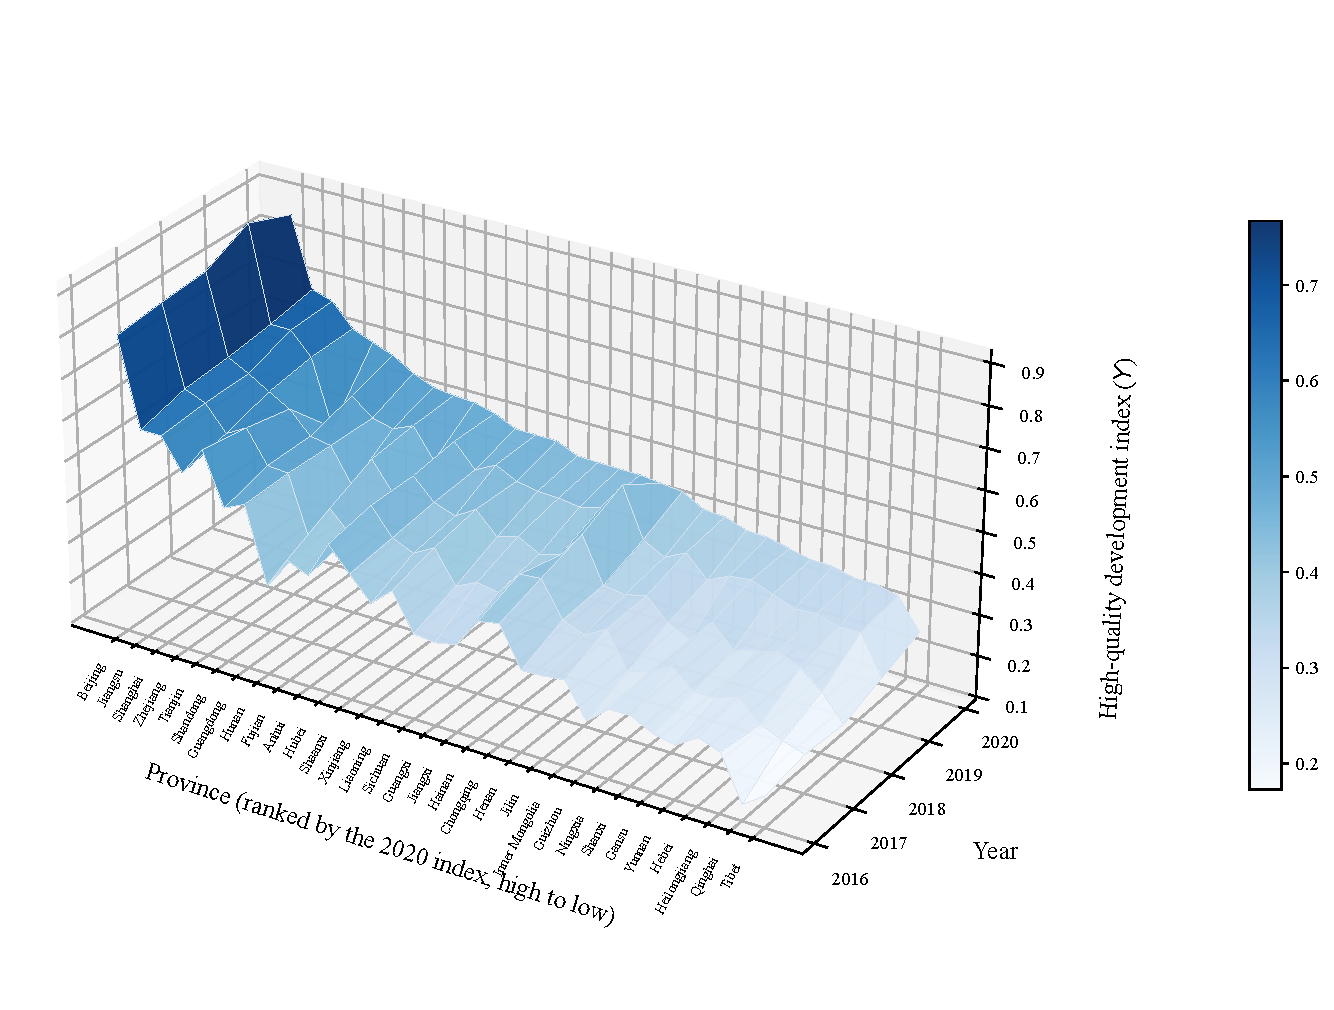
\includegraphics[width=0.90\textwidth]{figure1/Y_surface_province_year_English.pdf}
	\caption{Three-dimensional province--year surface of the high-quality
		economic development index $Y$. Provinces are ordered from high to low
		according to their 2020 index values. The horizontal ordering is
		rank-based rather than geographic.}
	\label{fig:y_surface}
\end{figure}

Figure~\ref{fig:y_surface} presents the three-dimensional province--year
surface of the high-quality economic development index, $Y$, during
2016--2020. Provinces are ordered from high to low according to their
2020 values of $Y$, while the other horizontal axis represents the year
and the vertical axis reports the index level.

Along the time dimension, the surface shifts upward from the earlier to
the later years, indicating a broad-based improvement in the level of
high-quality economic development during the sample period. The elevated
position of the later-year profiles suggests that this improvement was not
confined to a small subset of provinces, but instead reflected a relatively
widespread upward movement.

The cross-sectional profile reveals a pronounced but continuous ranking
gradient. An elevated ridge appears at the high-ranked end of the
provincial distribution, followed by a gradual decline toward the
low-ranked end. This pattern indicates persistent differences in
development quality across provinces. At the same time, the surface does
not separate into several sharply distinct plateaus, suggesting that
interprovincial heterogeneity is better characterized as a continuous
gradient than as extreme bipolarization.

This interpretation is consistent with the descriptive statistics reported
in the paper. The national mean of the high-quality development index
increased from 0.365 in 2016 to 0.462 in 2020, whereas the Dagum Gini
coefficient declined from 0.215 to 0.141. Thus, high-quality economic
development improved in aggregate while regional inequality decreased.
The decline in the Gini coefficient is consistent with relatively faster
improvement among lower-ranked provinces, which partially narrowed the gap
between the high- and low-performing regions.

The figure should nevertheless be interpreted with caution. Because the
province dimension is ordered according to the 2020 value of $Y$ rather
than geographic location, the plot is useful for describing temporal
evolution and differences in provincial rankings, but it does not, by
itself, establish geographically mediated spillovers or spatial
dependence. Accordingly, it should be viewed as a descriptive
rank-ordered province--year surface rather than a substitute for Moran's
$I$, a spatial Durbin model, or a formal spatial kernel-density estimate.



\subsection{DEA--Malmquist Agricultural TFP}

Total factor productivity (TFP) is conventionally defined as the ratio of
output to the bundle of all factor inputs \cite{liu1999}. In growth-accounting terms, TFP
growth is the residual component of output growth after removing the
contributions of observable inputs such as land, labor, and capital. The
principal measurement traditions are parametric, nonparametric, and index-
number approaches. Although they differ in assumptions and implementation,
all three seek to distinguish output changes from those attributable to
measured input accumulation.

The Solow-residual (growth-accounting) approach used in influential work on
Chinese agriculture by Fan and Zhang \cite{fan2002} is transparent, but it
relies on perfect competition and constant returns to scale to interpret
factor-income shares as output elasticities. When these assumptions fail,
the residual may capture scale effects, market distortions, or errors in
factor shares as well as productivity change. Its direction of bias is not
determined by returns to scale alone. The residual also does not
unambiguously identify the sources of productivity growth and requires
accurate factor-income shares, including land rents
and labor compensation, which are difficult to observe consistently across
provinces.

Stochastic frontier analysis (SFA) provides a parametric alternative. Yu,
Guo, and Zhang \cite{yu2011} combine an SFA production function with a
Shapley-value inequality decomposition to study the evolution and
determinants of regional agricultural labor-productivity differences.
SFA, however, requires assumptions about the production function and the
distributions of noise and inefficiency. These modeling choices matter for
regional agricultural productivity comparisons \cite{gao2015}. Conventional
production-function SFA typically models a single aggregate output, whereas
agriculture jointly produces grain,
cotton, oilseeds, livestock, and other outputs. Researchers must therefore
either aggregate outputs into a value measure or specify a multi-output
distance-function model, introducing additional aggregation or specification
choices.

We therefore adopt the DEA--Malmquist framework of
F\"are et al. \cite{fare1994}. It is a nonparametric frontier method that does
not impose a functional form and naturally accommodates multiple inputs and
outputs in principle, without requiring factor-income-share weights.
However, our implementation retains constant returns to scale and uses a
single aggregate monetary output. As a deterministic frontier method, DEA
also remains sensitive to measurement error and influential observations;
the choice does not remove these limitations.

Each province is treated as a decision-making unit. The input vector includes pesticide use, agricultural machinery power, agricultural diesel use, fertilizer use, and plastic-film use; the output is the gross value of agriculture, forestry, animal husbandry, and fisheries. Under an output orientation and constant returns to scale, the distance function is
\begin{equation}
D_{0}^{t}(x^{t},y^{t})=\min\left\{\theta:\left(x^{t},\frac{y^{t}}{\theta}\right)\in S^{t}\right\}.
\label{eq:distance}
\end{equation}
The adjacent-period Malmquist productivity index is
\begin{equation}
M_{0}^{t,t+1}=\left[
\frac{D_{0}^{t}(x^{t+1},y^{t+1})}{D_{0}^{t}(x^{t},y^{t})}
\frac{D_{0}^{t+1}(x^{t+1},y^{t+1})}{D_{0}^{t+1}(x^{t},y^{t})}
\right]^{1/2}.
\label{eq:malmquist}
\end{equation}
Because the Malmquist index is a growth index rather than an absolute productivity level, we define 2016 as the base period and normalize its value to one for every province; subsequent observations are cumulative chained products of the adjacent-period Malmquist indices. The resulting provincial trajectories are shown in Figure~\ref{fig:x_heatmap}.
\begin{equation}
TFP_{i,2016}=1,\qquad TFP_{i,t}=TFP_{i,t-1}M_{0,i}^{t-1,t}\quad (t=2017,\ldots,2020).
\label{eq:cumulative}
\end{equation}

\begin{figure}[H]
\centering
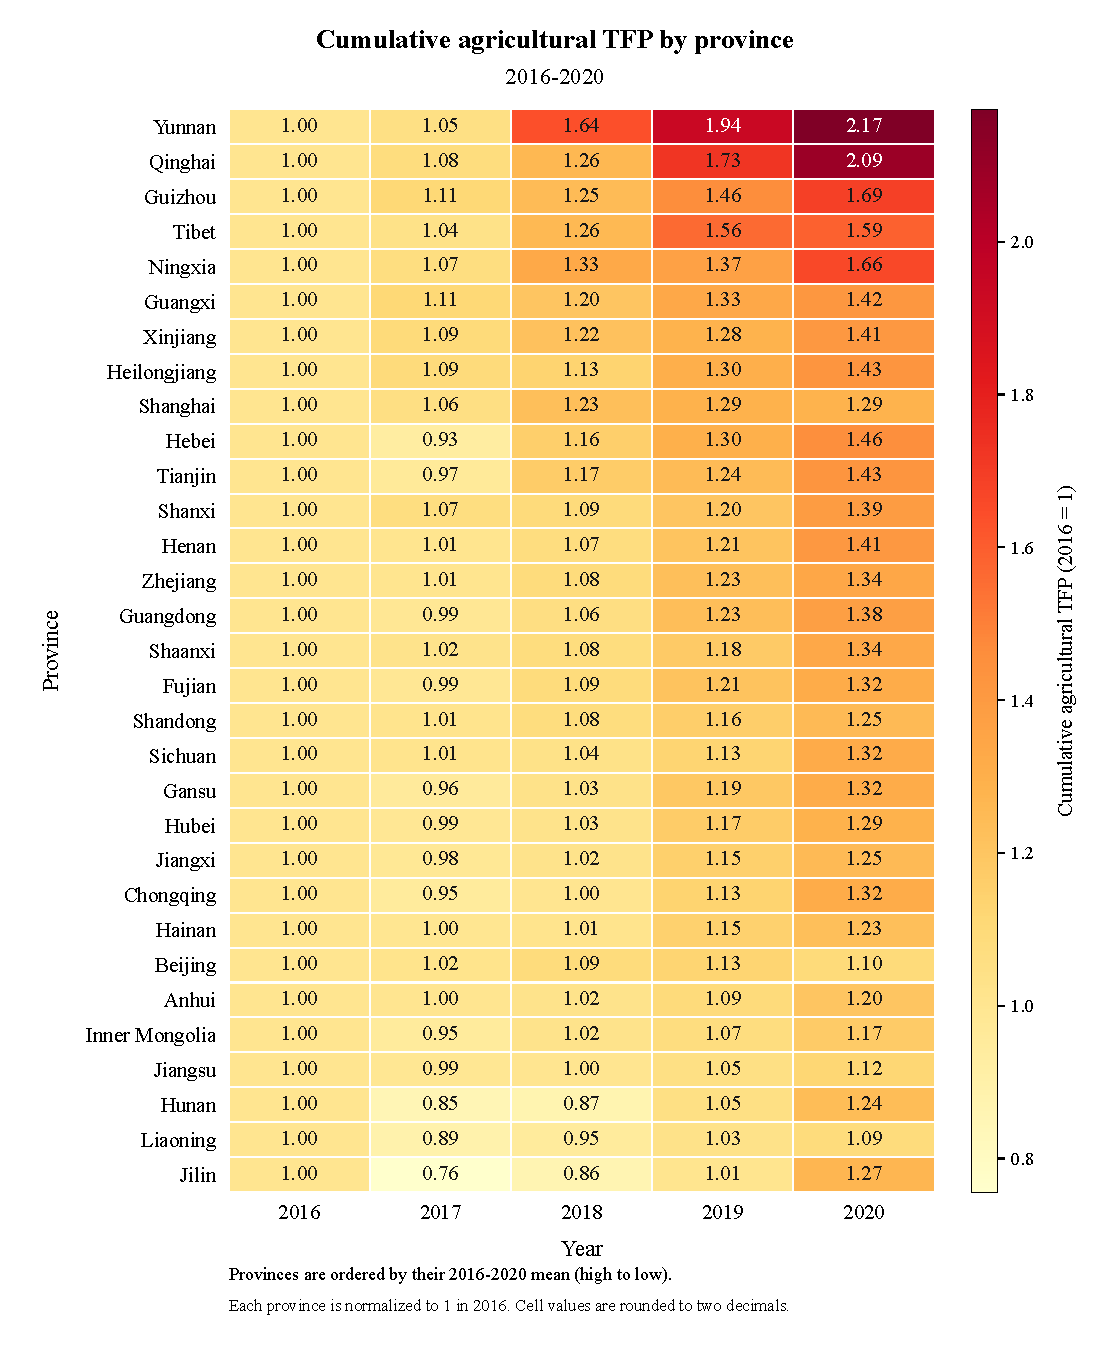
\includegraphics[width=0.86\textwidth]{figure1/X_cumulative_TFP_heatmap_English.pdf}
\caption{Cumulative agricultural total factor productivity (TFP) by province, 2016--2020. Each province is normalized to one in 2016; subsequent values are chained cumulative products of the adjacent-period Malmquist indices. Provinces are ordered by their sample-period mean cumulative TFP, from high to low.}
\label{fig:x_heatmap}
\end{figure}

The heatmap reports the cumulative Agricultural TFP index, $X$, for 31
provincial-level regions from 2016 to 2020. Each province is normalized
to its own 2016 base period, which is assigned a value of one. The
unweighted cross-provincial mean was 1.001 in 2017 and subsequently rose
to 1.109, 1.245, and 1.386 in 2018, 2019, and 2020, respectively. Fourteen
provinces remained below their own base-period level in 2017, and this
number fell to three in 2018; from 2019 onward, all provinces exceeded
their respective base values. By 2020, the mean cumulative gain was
38.65\%, while the median gain was 32.32\%, indicating broad-based
productivity improvement during the latter part of the sample period.

The magnitude of cumulative growth differed substantially across
provinces. In 2020, the index reached 2.173 in Yunnan and 2.092 in Qinghai,
whereas it was 1.086 in Liaoning, 1.096 in Beijing, and 1.119 in Jiangsu.
The trajectories were not uniformly monotonic: between 2019 and 2020,
the index declined by approximately 3.08\% in Beijing and 0.30\% in
Shanghai. Shanghai is annotated as 1.29 in both years because the figure
rounds values to two decimal places; this rounding does not imply that
the index was unchanged.

Because each province is normalized to its own base period, the heatmap
describes cumulative productivity changes relative to that province's
initial level and cannot establish an interprovincial ranking of absolute
productivity. The 38.65\% figure is likewise an unweighted mean of
province-specific cumulative gains. Moreover, a heatmap with rows ordered
by the index does not by itself establish geographic clustering or spatial
dependence. We therefore use several complementary methods below to
provide an initial examination of these spatial features.

\subsection{Distribution and regional inequality}

Kernel density estimation is used to visualize distributional movement:
\begin{equation}
\widehat f_h(x)=\frac{1}{nh}\sum_{i=1}^{n}K\left(\frac{x-x_i}{h}\right).
\label{eq:kde}
\end{equation}
Here, $n$ is the number of provincial observations in the relevant year and
region, $h$ is the bandwidth, and $K(u)=(2\pi)^{-1/2}\exp(-u^2/2)$ is the
Gaussian kernel. We use Scott's rule, $h=s n^{-1/5}$, where $s$ is the sample
standard deviation, and estimate each year or region separately. Curves are
displayed over the feasible index range without a boundary correction.
The curves are descriptive estimates of marginal
distributions, not tests of geographic dependence. Cumulative TFP has zero
cross-sectional variance in the 2016 base year, so that year is represented
by a vertical line at one rather than a density curve.
The Dagum Gini coefficient \cite{dagum1997} is decomposed into within-region, net between-region, and transvariation components. Because this model contains more than three linked sub-equations, the components share one equation number:
\begin{equation}
\begin{aligned}
G&=\frac{\sum_j\sum_h\sum_i\sum_r|x_{ji}-x_{hr}|}{2n^2\bar x},\\
G&=G_w+G_{nb}+G_t,\\
G_w&=\sum_jG_{jj}p_js_j,\\
G_{nb}&=\sum_{j>h}G_{jh}D_{jh}(p_js_h+p_hs_j),\\
G_t&=\sum_{j>h}G_{jh}(1-D_{jh})(p_js_h+p_hs_j).
\end{aligned}
\label{eq:dagum}
\end{equation}

\subsection{Spatial autocorrelation}

The baseline spatial weights matrix is a row-standardized binary contiguity matrix. Hainan is linked to Guangdong to avoid an island observation; this bridge is an explicit modeling assumption. Global Moran's I is
\begin{equation}
I=\frac{n}{S_0}\frac{\sum_{i=1}^{n}\sum_{j=1}^{n}w_{ij}(x_i-\bar x)(x_j-\bar x)}{\sum_{i=1}^{n}(x_i-\bar x)^2},
\qquad S_0=\sum_i\sum_jw_{ij}.
\label{eq:globalmoran}
\end{equation}
The local Moran statistic is
\begin{equation}
I_i=z_i\sum_{j=1}^{n}w_{ij}z_j.
\label{eq:localmoran}
\end{equation}
Inference uses 999 random permutations. Local clusters are classified as high--high (HH), low--low (LL), low--high (LH), or high--low (HL), with significance assessed at $p<0.05$.

\subsection{Coupling coordination model}

Following the methodological cautions of Wang et al. \cite{wang2021},
we distinguish coupling strength from the development levels of the
two subsystems and examine sensitivity to normalization and weighting.
Coupling coordination is a descriptive measure of joint development;
it does not establish that one subsystem causally improves the other.

Agricultural TFP is standardized over the full 2016--2020 sample and shifted by $\varepsilon=0.01$ to prevent a zero subsystem score. Let $U_1$ denote standardized Agricultural TFP and $U_2$ the high-quality development index. The three linked components share one model number:
\begin{equation}
\begin{aligned}
C_{it}&=\frac{2\sqrt{U_{1,it}U_{2,it}}}{U_{1,it}+U_{2,it}},\\
T_{it}&=\alpha U_{1,it}+\beta U_{2,it},\qquad \alpha=\beta=0.5,\\
D_{it}&=\sqrt{C_{it}T_{it}}.
\end{aligned}
\label{eq:ccd}
\end{equation}
Values of $D$ are divided into ten equal-width categories from extreme imbalance ($0\le D<0.1$) to high coordination ($0.9\le D\le 1$). Robustness checks vary the zero shift, normalization rule, and subsystem weights.

\subsection{Panel, spatial, threshold, and Markov models}

The baseline two-way fixed-effects model is
\begin{equation}
\ln Y_{it}=\beta\ln TFP_{it}+\bm{\gamma}'\bm{X}_{it}+\mu_i+\tau_t+\varepsilon_{it},
\label{eq:fe}
\end{equation}
where $\bm{X}_{it}$ contains log population density and the primary-sector
share. Population density is resident population divided by administrative
land area; its expected sign is ambiguous because agglomeration benefits may
be offset by congestion and land pressure. The primary-sector share is
100 times primary-industry value added divided by GDP, measured in
percentage points, and captures industrial
structure and dependence on agriculture. A larger share can also signal
dependence on relatively less diversified activities, so its conditional sign
is expected to be negative or zero rather than unambiguously positive. The province effects $\mu_i$
absorb time-invariant provincial characteristics, while the year effects
$\tau_t$ absorb common annual shocks. The disturbance is $\varepsilon_{it}$.
All baseline specifications use the same 155 observations. Province-clustered
standard errors use the CR1 finite-sample multiplier
$G(N-1)/[(G-1)(N-k)]$, where $G$ is the number of provinces, $N$ is the number
of observations, and $k$ is the full design-matrix rank including fixed
effects. Tests and confidence intervals use a $t_{G-1}$ reference
distribution. In the log--log specification, $\beta$
is the conditional elasticity of the high-quality development index with
respect to cumulative agricultural TFP.

The spatial Durbin specification is
\begin{equation}
\ln Y_{it}=\rho W\ln Y_{it}+\beta\ln TFP_{it}+\bm{\gamma}'\bm{X}_{it}
+\theta W\ln TFP_{it}+\bm{\eta}'W\bm{X}_{it}+\mu_i+\tau_t+\varepsilon_{it}.
\label{eq:sdm}
\end{equation}
The feedback-adjusted marginal-effect matrix for Agricultural TFP is
\begin{equation}
\frac{\partial \bm y}{\partial \bm x'}=(I_n-\rho W)^{-1}(\beta I_n+\theta W).
\label{eq:impact}
\end{equation}

With log GDP per capita $q_{it}$ as the threshold variable, the single-threshold model is
\begin{equation}
\ln Y_{it}=\beta_1\ln TFP_{it}\mathbb{I}(q_{it}\le\gamma)
+\beta_2\ln TFP_{it}\mathbb{I}(q_{it}>\gamma)
+\bm{\gamma}'\bm{X}_{it}+\mu_i+\tau_t+\varepsilon_{it}.
\label{eq:threshold}
\end{equation}

Candidate thresholds are searched over the 15th--85th percentiles of log GDP
per capita to retain observations on both sides of the split. The threshold
test uses 499 province-level wild-cluster bootstrap replications. The
likelihood-ratio confidence set consists of candidate values satisfying
$LR(\gamma)\leq 7.35$.

Following the spatial Markov approach of Rey \cite{rey2001}, each year's high-quality development score is assigned to one of four quartile states. The transition probability is
\begin{equation}
p_{ij}^{(k)}=\Pr\left(s_{i,t+1}=j\mid s_{it}=i,\;\ell_{it}=k\right)
=\frac{n_{ij}^{(k)}}{\sum_{j=1}^{4}n_{ij}^{(k)}},
\label{eq:markov}
\end{equation}
where $\ell_{it}$ is a low-, middle-, or high-neighborhood state determined from the spatial lag. Matrix mobility is summarized by the Shorrocks index
\begin{equation}
M(P)=\frac{4-\operatorname{tr}(P)}{3}.
\label{eq:shorrocks}
\end{equation}
A permutation-based likelihood-ratio statistic tests whether the conditional matrices differ from the pooled matrix:
\begin{equation}
G=2\sum_k\sum_i\sum_j n_{ij}^{(k)}
\ln\left(\frac{p_{ij}^{(k)}}{p_{ij}}\right).
\label{eq:gtest}
\end{equation}

\section{Empirical results}

\subsection{Distribution dynamics and regional disparities}

\subsubsection{National distribution dynamics}

Figure~\ref{fig:kde_national} contrasts the national distributions of
cumulative agricultural TFP and high-quality economic development.
The TFP distribution shifts to the right after the common 2016 base year,
with annual means of 1.001, 1.109, 1.245, and 1.386 in 2017--2020.
Its main peak becomes lower and its dispersion increases: the provincial
standard deviation rises from 0.076 in 2017 to 0.245 in 2020.
An extended upper tail, reaching beyond two by 2020, indicates that some
provinces accumulated substantially larger productivity gains than others.
Because the index chains annual changes, this widening describes
heterogeneity in cumulative growth, not a ranking of absolute productivity
levels or evidence of an abrupt structural break.

\begin{figure}[H]
\centering
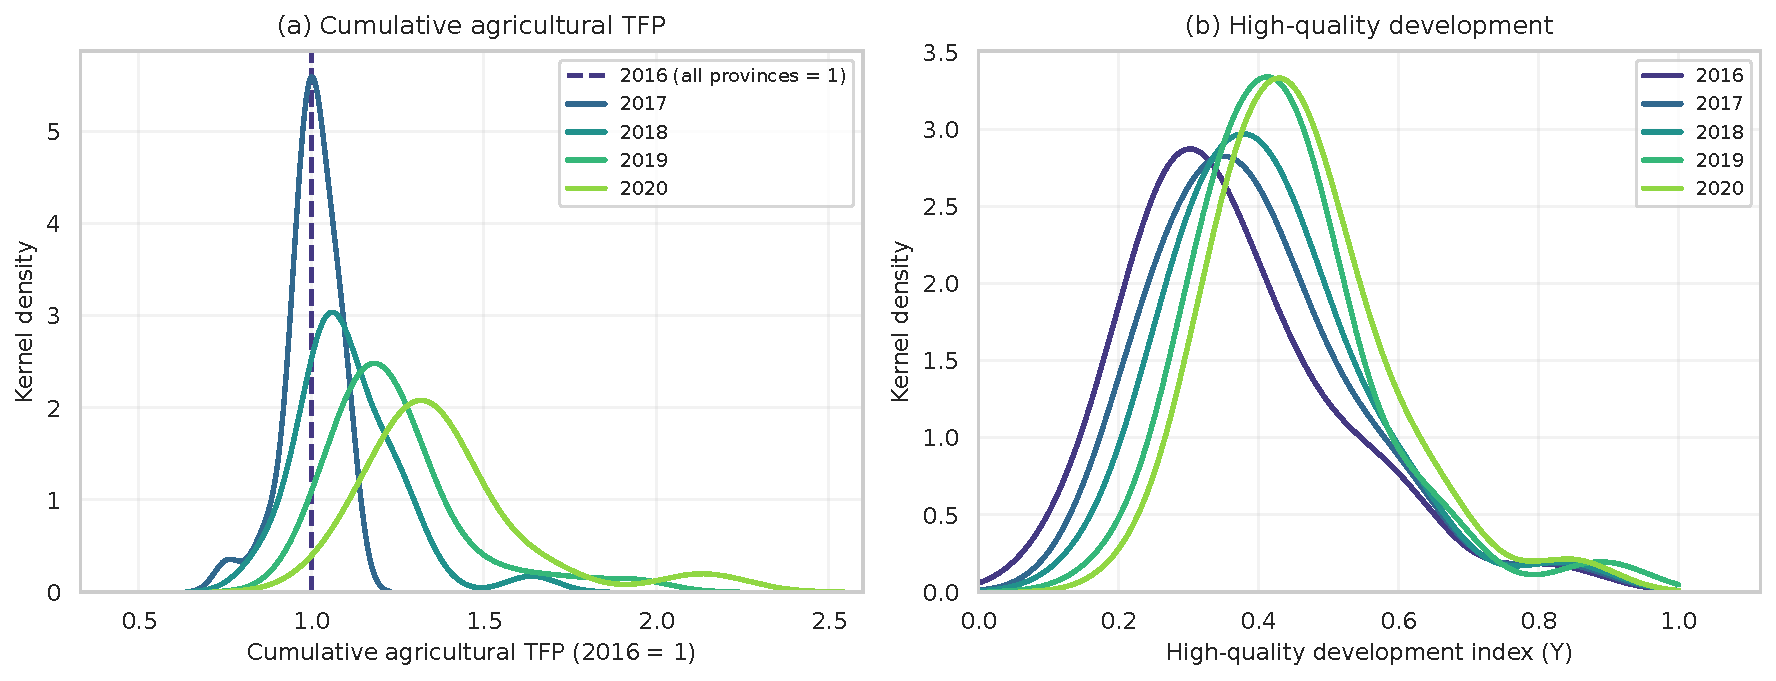
\includegraphics[width=\textwidth]{figure1/KDE_national_Y_TFP_2016_2020_English.pdf}
\caption{National kernel density estimates, 2016--2020: (\textbf{a}) cumulative agricultural TFP and (\textbf{b}) high-quality economic development. Gaussian kernels with Scott bandwidths are estimated separately for each year. The dashed line at one represents the 2016 TFP point mass, not an estimated density.}
\label{fig:kde_national}
\end{figure}

For high-quality development, the distribution also shifts rightward, but
its dispersion contracts. The provincial mean increases from 0.365 in
2016 to 0.462 in 2020, a gain of approximately 26.5\%, while the standard
deviation falls from 0.149 to 0.123. Later-year densities are generally more
concentrated around their main peak, although peak heights do not rise
monotonically. The persistent right tail indicates that leading provinces
remain ahead. Taken together, the estimates suggest an improvement in
development quality accompanied by narrower provincial differences.
Small shoulders should not be interpreted as distinct convergence clubs:
each annual cross-section contains only 31 observations, and the apparent
number of modes depends on the smoothing bandwidth.

\subsubsection{Regional distribution dynamics}

Figure~\ref{fig:kde_tfp_regions} disaggregates cumulative TFP into eastern,
central, and western regions. In 2017, regional means are 0.985, 0.967,
and 1.038, respectively, and the distributions overlap substantially.
The eastern distribution is relatively concentrated, while the central
distribution has a more pronounced lower tail. By 2018, the corresponding
means reach 1.084, 1.013, and 1.194. The western distribution shifts farther
to the right and develops a broader upper tail, a pattern that persists
in 2019, when regional means reach 1.185, 1.148, and 1.364.

\begin{figure}[H]
\centering
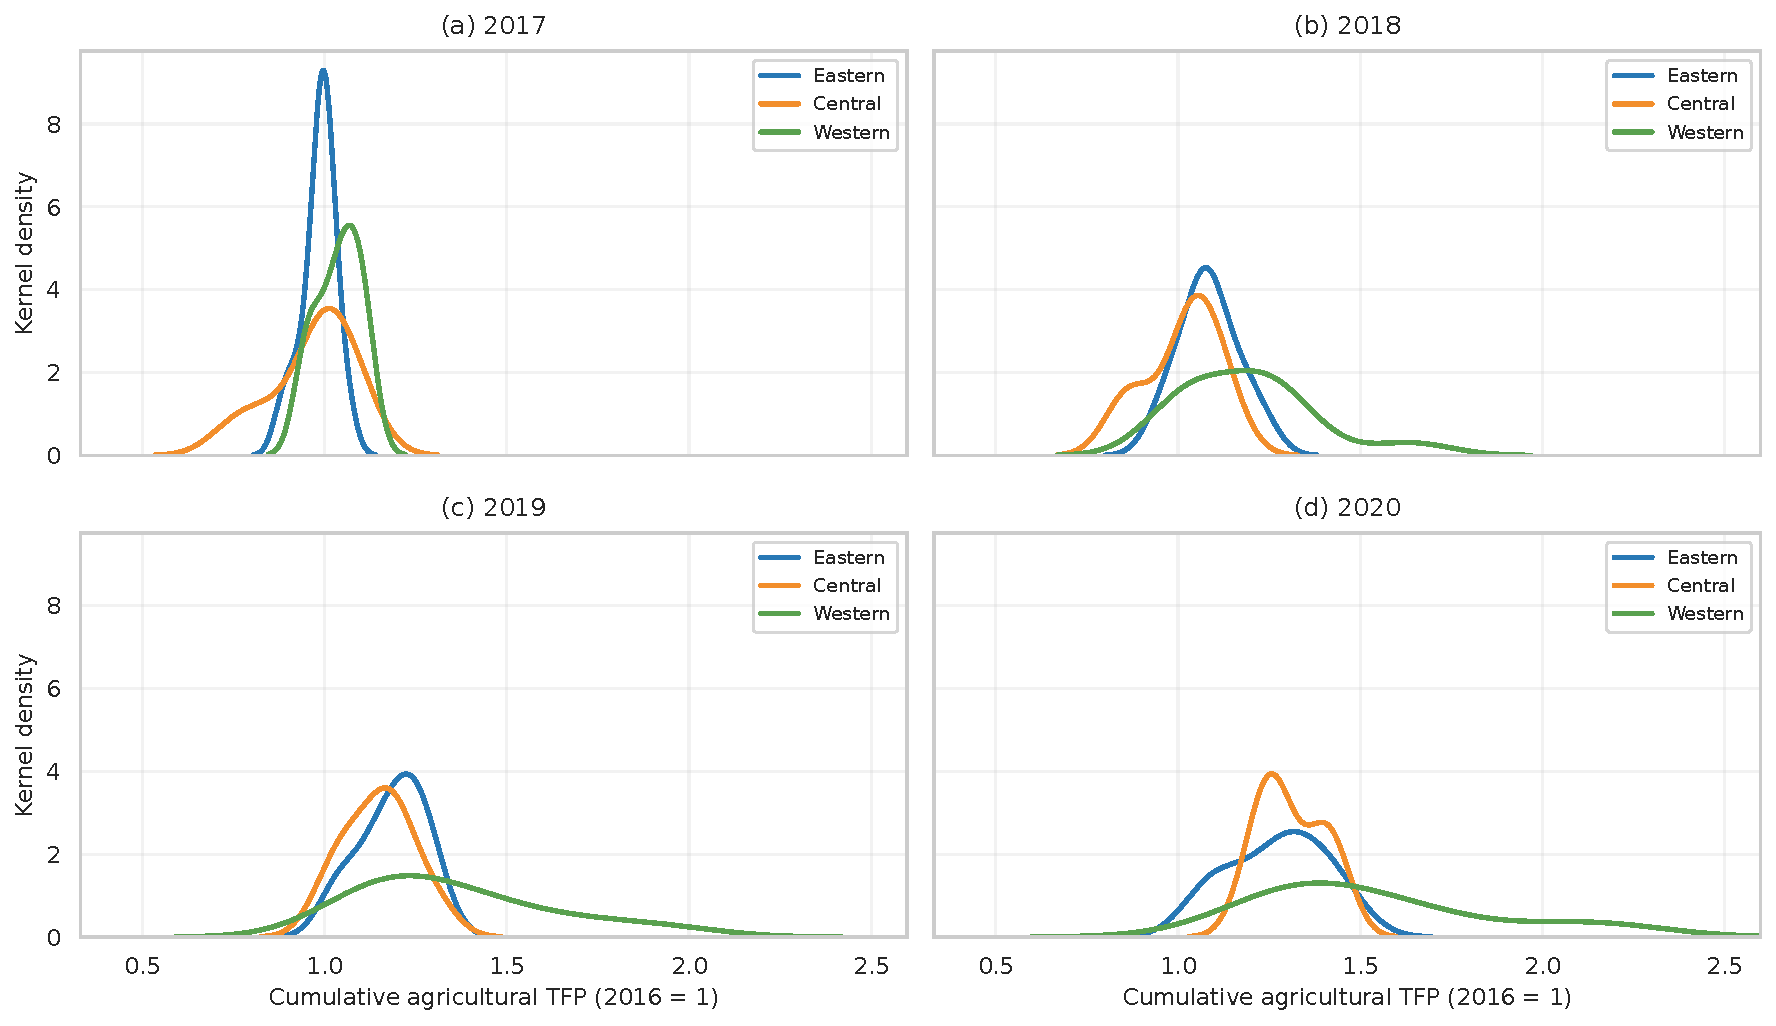
\includegraphics[width=\textwidth]{figure1/KDE_regional_TFP_English.pdf}
\caption{Regional kernel density estimates of cumulative agricultural TFP, 2017--2020. Eastern, central, and western samples contain 11, 8, and 12 provinces, respectively. The common base year 2016 is omitted because all provincial observations equal one. Bandwidths are selected separately by region and year.}
\label{fig:kde_tfp_regions}
\end{figure}

In 2020, mean cumulative TFP is 1.272 in the east, 1.311 in the center,
and 1.542 in the west. Within-region standard deviations are 0.129,
0.086, and 0.316, respectively. Thus, the west combines the largest
average cumulative gain with the greatest dispersion, whereas central
provinces follow more similar growth paths. These comparisons concern
changes relative to each province's own base year. They do not establish
that western provinces have higher absolute productivity or identify
whether differences arise from technology, efficiency, input adjustment,
or changes in the estimated frontier.

Figure~\ref{fig:kde_y_regions} shows a different regional ordering for
high-quality development. The eastern distribution remains farther to
the right, while the central distribution generally lies between those
of the east and west. From 2016 to 2020, regional means increase from
0.502 to 0.565 in the east, from 0.316 to 0.432 in the center, and from
0.272 to 0.387 in the west. The eastern distribution is comparatively
broad, indicating substantial internal differences despite its higher mean.
The central distribution is more concentrated. Occasional shoulders or
plateaus in the western curves are only suggestive of internal
heterogeneity, given the small regional samples.

\begin{figure}[H]
\centering
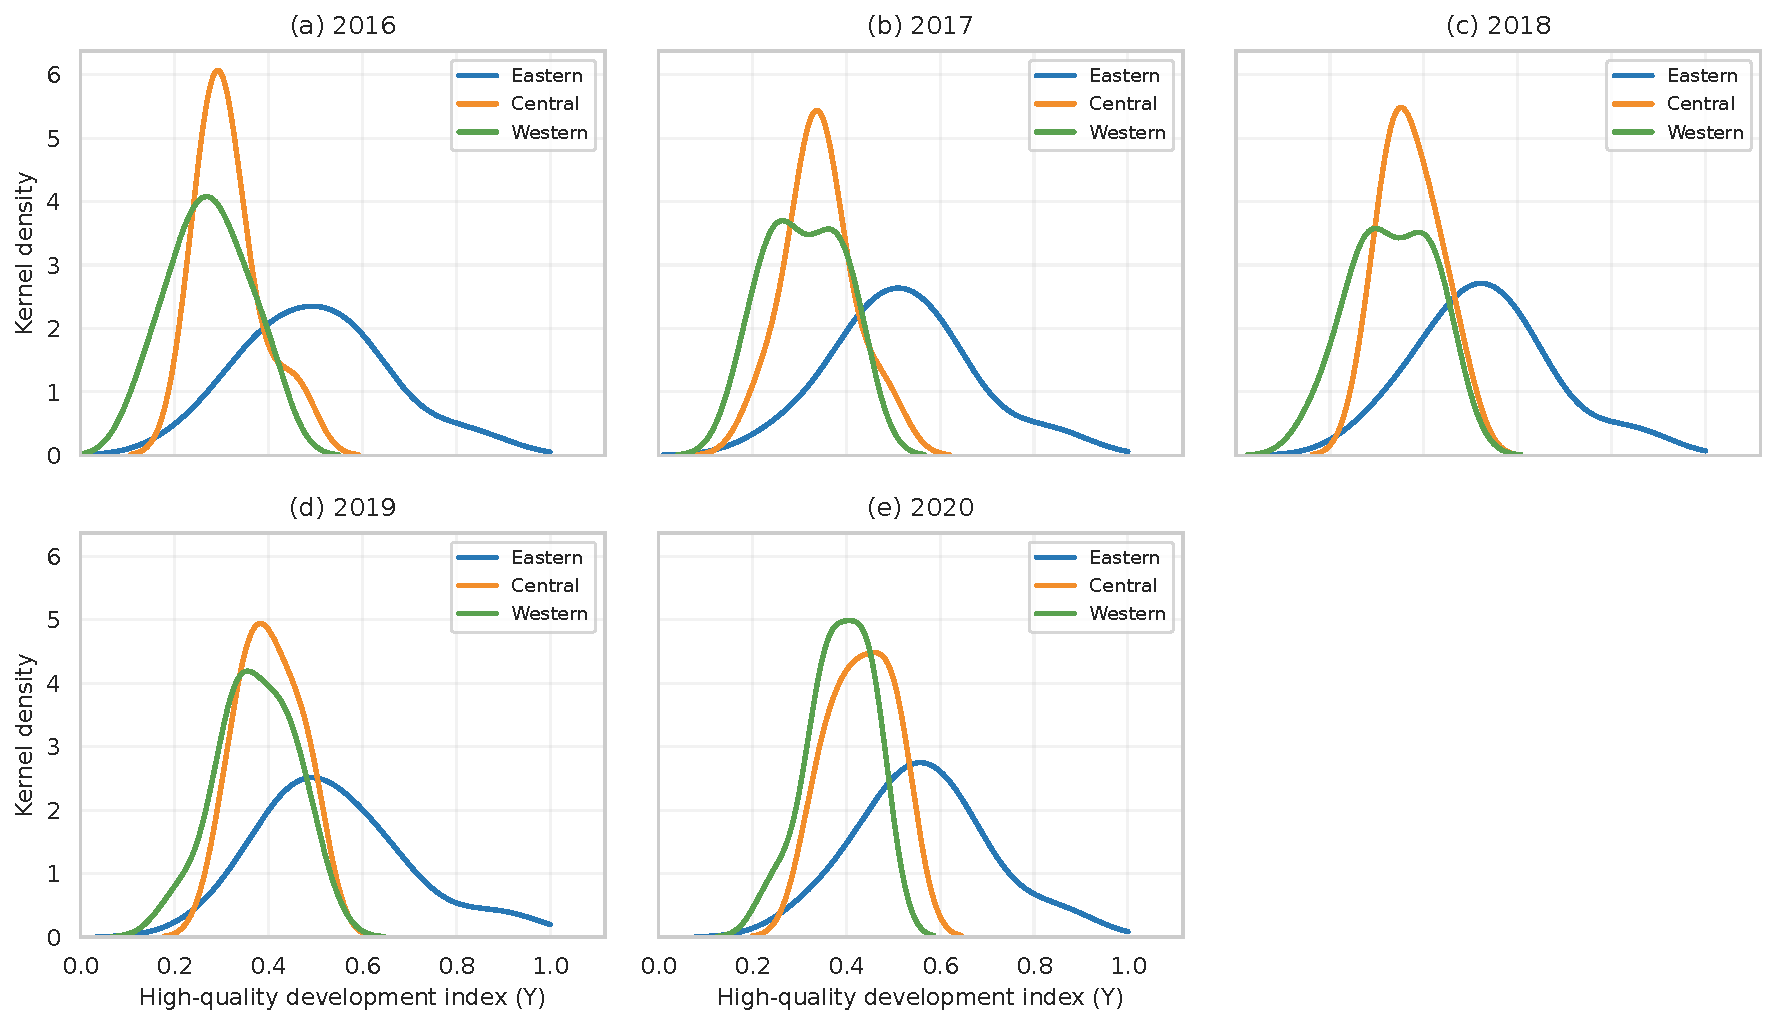
\includegraphics[width=\textwidth]{figure1/KDE_regional_Y_English.pdf}
\caption{Regional kernel density estimates of the high-quality economic development index, 2016--2020. Regional definitions and Gaussian-kernel estimation follow Figure~\ref{fig:kde_tfp_regions}. The panels use common axes to facilitate comparisons over time.}
\label{fig:kde_y_regions}
\end{figure}

The east--west mean gap narrows from 0.229 to 0.178, and the
east--central gap falls from 0.186 to 0.132. These movements are
consistent with faster improvement in the central and western regions,
although the eastern lead persists. Regional density comparisons are
descriptive and do not themselves establish spatial dependence or spillovers.
We next quantify the sources of inequality with the Dagum decomposition.

\subsubsection{Dagum inequality decomposition}

\begin{table}[H]
\centering
\caption{National means and Dagum Gini coefficients for $Y$ and cumulative Agricultural TFP $X$, 2016--2020}
\label{tab:distribution}
\small
\begin{tabular}{ccccc}
\toprule
Year & Mean $Y$ & Gini $Y$ & \shortstack{Mean $X$\\(cumulative TFP)} & Gini cumulative TFP \\
\midrule
2016 & 0.365 & 0.215 & 1.000 & 0.000 \\
2017 & 0.394 & 0.192 & 1.001 & 0.040 \\
2018 & 0.414 & 0.174 & 1.109 & 0.067 \\
2019 & 0.440 & 0.152 & 1.245 & 0.078 \\
2020 & 0.462 & 0.141 & 1.386 & 0.085 \\
\bottomrule
\end{tabular}
\end{table}

\begin{figure}[H]
\centering
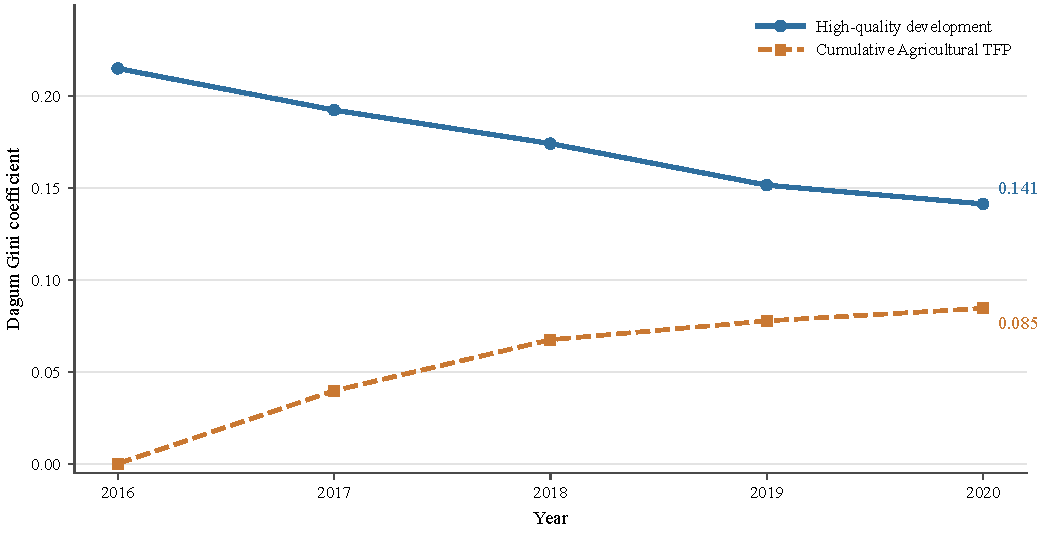
\includegraphics[width=0.82\textwidth]{figures/Figure01_Dagum_Gini_trends.pdf}
\caption{Evolution of interprovincial Dagum Gini coefficients. The 2016 Agricultural TFP coefficient is zero by construction because cumulative TFP shares a common base.}
\label{fig:dagum}
\end{figure}

Table~\ref{tab:distribution} and Figure~\ref{fig:dagum} document contrasting
distributional changes in high-quality economic development and cumulative
agricultural TFP across provinces. Between 2016 and 2020, the equally weighted
provincial mean of the high-quality development index increased from 0.365
to 0.462, or approximately 26.5\%, while its national Gini coefficient declined
in every year, from 0.215 to 0.141, a reduction of approximately 34.3\%.
Improvements in average development quality thus coincided with lower relative
dispersion across provinces. Mean cumulative agricultural TFP increased from
its base value of one to 1.386, but its national Gini coefficient rose from
0.040 in 2017 to 0.085 in 2020. This indicates increasingly uneven cumulative
productivity growth, reflecting wider differences in the gains provinces
achieved relative to their respective base years.

\begin{figure}[H]
\centering
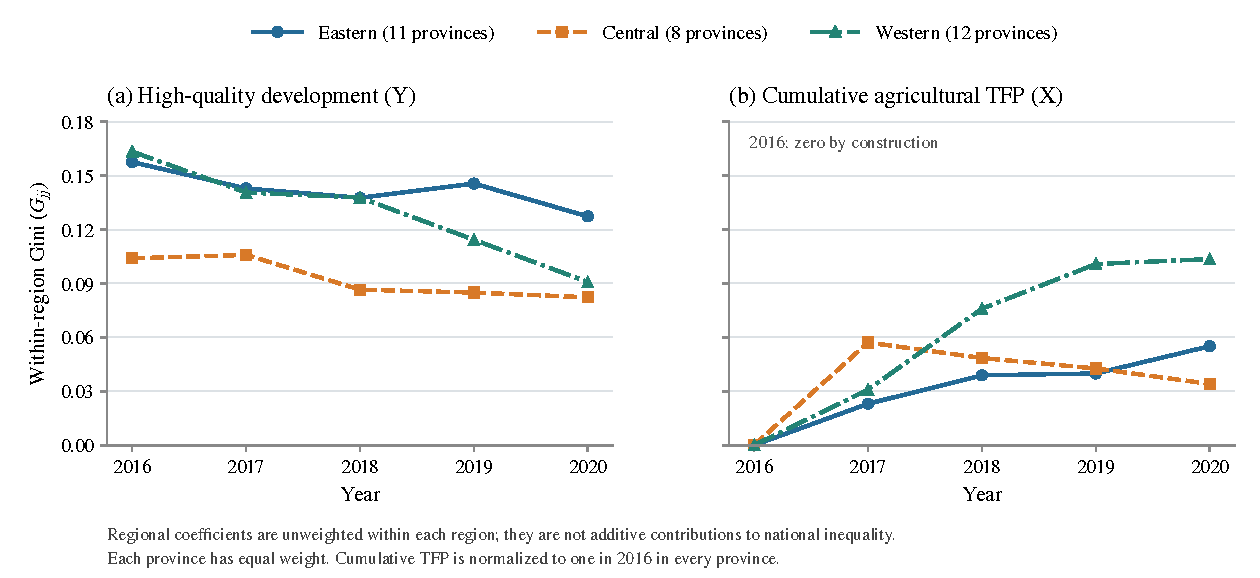
\includegraphics[width=\textwidth]{figures/Dagum_within_region_Gini_English.pdf}
\caption{Within-region Dagum Gini coefficients, 2016--2020: (\textbf{a}) high-quality economic development and (\textbf{b}) cumulative agricultural TFP. Eastern, central, and western China contain 11, 8, and 12 sampled provinces, respectively. Provinces receive equal weight within each region. The regional coefficients are not additive contributions to national inequality. TFP coefficients are zero in 2016 because every province shares the base value of one.}
\label{fig:dagum_within}
\end{figure}

The within-region results reveal substantial heterogeneity beneath these
national trends. As shown in Figure~\ref{fig:dagum_within}(a), the Gini
coefficients for high-quality development declined from 0.158 to 0.127 in
eastern China, from 0.104 to 0.082 in central China, and from 0.163 to 0.091 in
western China between 2016 and 2020. The western region recorded the largest
reduction, approximately 44.4\%, and its coefficient declined throughout the
sample period. Changes elsewhere were less uniform: the eastern coefficient
temporarily increased in 2019, while the central coefficient edged upward in
2017. Improvements were therefore not fully synchronized across regions.
By 2020, within-region inequality was highest in the east and lowest in the
center. Together with the east's higher mean development index, this pattern
indicates that a higher regional average need not imply a more even
distribution of development quality within the region.

Within-region changes in cumulative agricultural TFP were markedly different.
Figure~\ref{fig:dagum_within}(b) shows that, between 2017 and 2020, the eastern
and western Gini coefficients increased from 0.023 to 0.055 and from 0.031 to
0.104, respectively. The central coefficient instead declined from 0.057 to
0.034. Faster average cumulative productivity growth in western China thus
coexisted with widening differences among its provinces, indicating that gains
were unevenly distributed. In central China, cumulative gains became more
similar across provinces. The increase in national TFP inequality consequently
does not reflect a uniform widening of inequality within all three regions.

\begin{figure}[H]
\centering
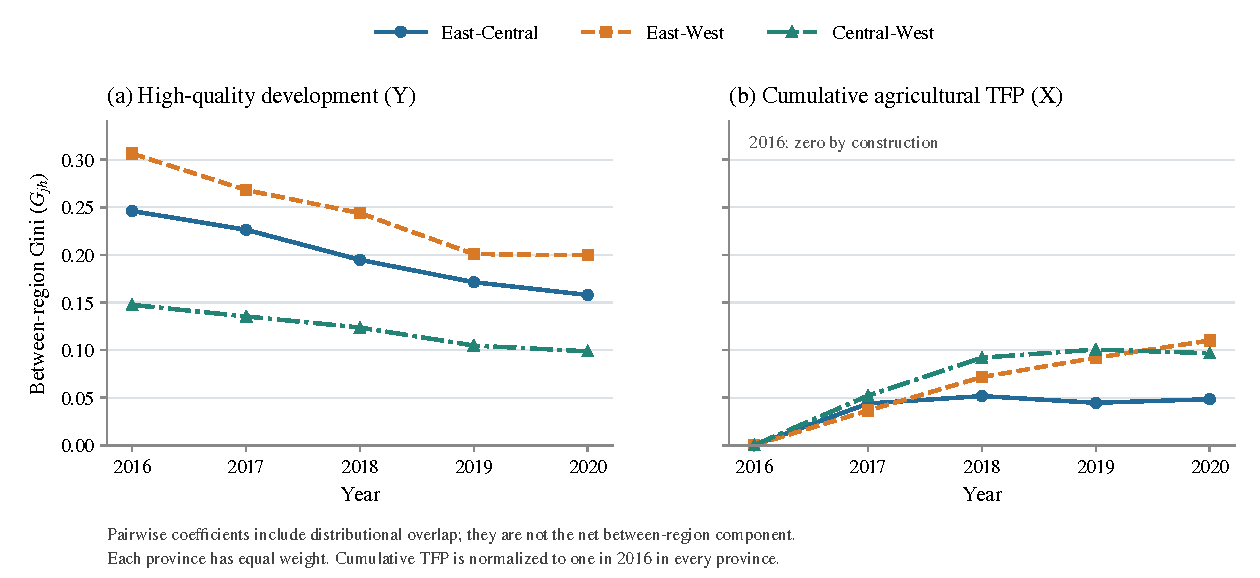
\includegraphics[width=\textwidth]{figures/Dagum_between_region_Gini_English.pdf}
\caption{Pairwise between-region Dagum Gini coefficients, 2016--2020: (\textbf{a}) high-quality economic development and (\textbf{b}) cumulative agricultural TFP. Each coefficient summarizes standardized absolute differences across provincial pairs belonging to the two indicated regions. These coefficients include distributional overlap and are distinct from the net between-region component of national inequality. Regional definitions follow Figure~\ref{fig:dagum_within}.}
\label{fig:dagum_between}
\end{figure}

The pairwise between-region results provide complementary evidence.
Figure~\ref{fig:dagum_between}(a) shows that the east--west, east--central, and
central--west Gini coefficients for high-quality development declined from
0.307, 0.246, and 0.147 in 2016 to 0.200, 0.158, and 0.099 in 2020, respectively.
All three declined in every year, although the east--west coefficient remained
the largest and the central--west coefficient the smallest. Regional
distributions thus became less disparate without eliminating the established
ordering of pairwise differences. For cumulative agricultural TFP,
Figure~\ref{fig:dagum_between}(b) shows a persistent increase in the east--west
coefficient, from 0.036 in 2017 to 0.110 in 2020, when it became the largest
pairwise disparity. The central--west coefficient increased from 0.052 to
0.097, with a modest decline after reaching approximately 0.101 in 2019, while
the east--central coefficient fluctuated at a lower level. The regional
divergence in cumulative productivity growth was therefore especially
pronounced between western China and the other regions. These pairwise
coefficients summarize differences across all cross-region provincial pairs;
they are distinct from both differences in regional means and the net
between-region component of the national decomposition.

\begin{figure}[H]
\centering
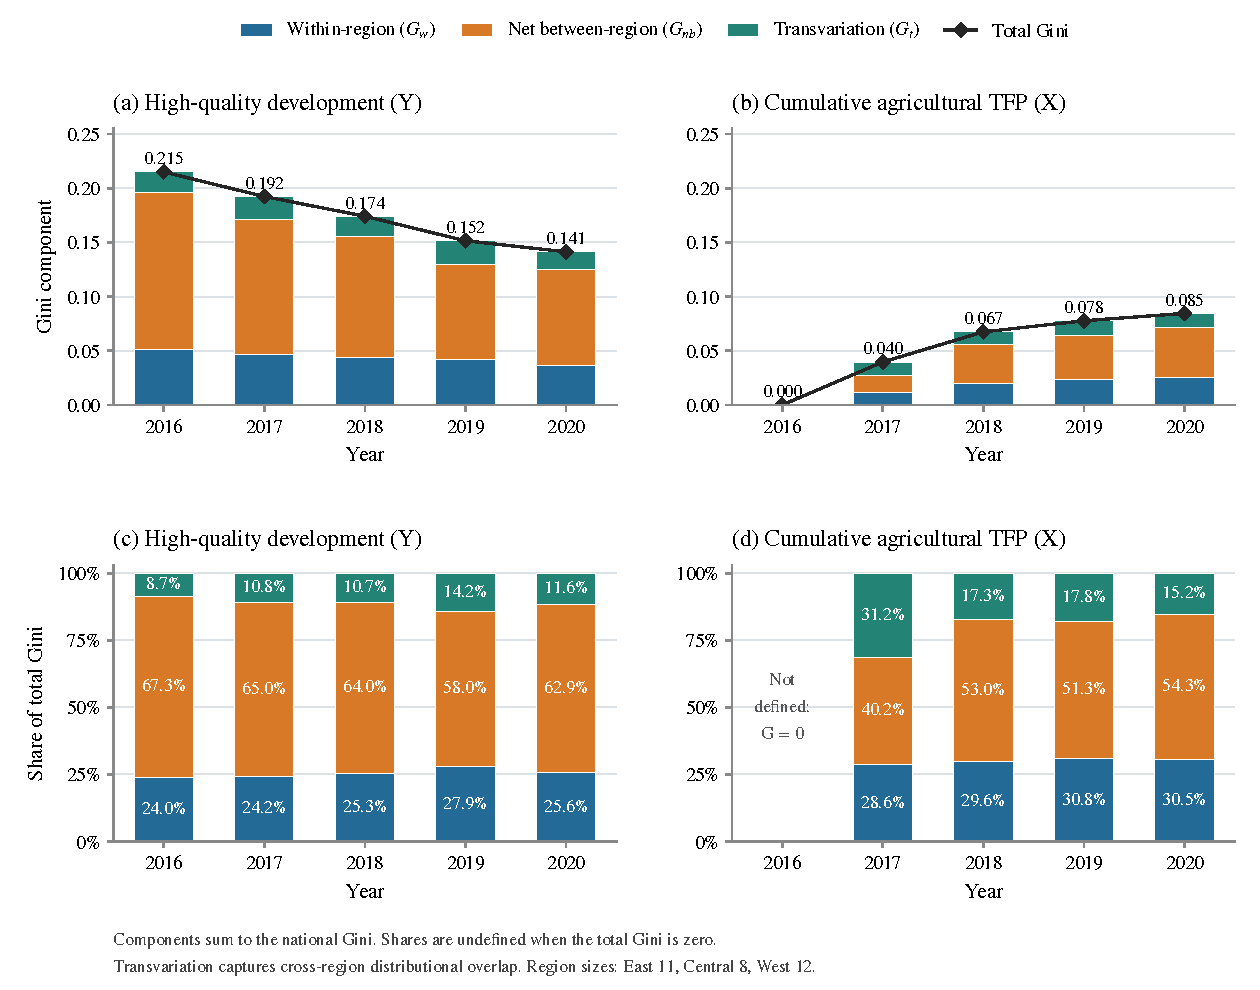
\includegraphics[width=\textwidth]{figures/Dagum_sources_decomposition_English.pdf}
\caption{Sources of national Dagum inequality: (\textbf{a},\textbf{b}) absolute component values and (\textbf{c},\textbf{d}) percentage contributions for high-quality economic development and cumulative agricultural TFP. The within-region, net between-region, and transvariation components sum to the national Gini. Transvariation captures cross-region distributional overlap. Contributions are undefined for TFP in 2016 because total inequality is zero. All calculations use equal provincial weights.}
\label{fig:dagum_sources}
\end{figure}

Figure~\ref{fig:dagum_sources} decomposes national inequality into within-region,
net between-region, and transvariation components. For high-quality development,
net between-region inequality accounted for 57.95--67.30\% of the national Gini
and remained its largest component throughout the sample period. Between 2016
and 2020, this component declined from 0.1448 to 0.0889, compared with reductions
from 0.0515 to 0.0361 in the within-region component and from 0.0188 to 0.0163
in transvariation. Under the decomposition identity, these changes account for
approximately 75.81\%, 20.88\%, and 3.31\% of the decline in the national Gini,
respectively. The narrowing of national inequality was therefore predominantly
associated with a reduction in its net between-region component. This is an
accounting attribution rather than evidence identifying the causal effects of
specific policies or economic mechanisms. Moreover, the net between-region
component increased slightly between 2019 and 2020, showing that a continued
decline in aggregate inequality need not involve simultaneous reductions in
every component.

For cumulative agricultural TFP, the net between-region component increased
from 0.0159 in 2017 to 0.0459 in 2020, while the within-region component increased
from 0.0113 to 0.0258. These changes account for approximately 66.71\% and
32.16\% of the increase in the national Gini, respectively. The net
between-region share rose, with some intermediate fluctuation, from 40.20\% to
54.28\%, indicating a greater relative importance of differences between
regional distributions by the end of the sample. The transvariation share
declined from 31.22\% to 15.24\%, although its absolute component increased
slightly, from approximately 0.0124 to 0.0129. The declining share therefore
reflects faster growth in the other components and should not be interpreted
as the disappearance of distributional overlap. Contribution shares are
undefined for cumulative TFP in 2016 because the national Gini is zero;
Figure~\ref{fig:dagum_sources} explicitly marks this case.

Taken together, these results indicate that the narrowing of disparities in high-quality economic development occurred both within and between regions, whereas the widening disparities in cumulative agricultural TFP primarily reflected an enlarged net between-region component, accompanied by rising within-region inequality in eastern and western China. This contrast suggests that cumulative productivity growth and comprehensive development quality follow distinct regional distributional trajectories and do not necessarily generate the same spatial pattern. The Dagum decomposition identifies the sources of distributional inequality but does not directly reveal whether provinces with similar or dissimilar levels are spatially clustered. Therefore, the following analysis employs global and local Moran’s I statistics to test for spatial autocorrelation and to identify potential high-high, low-low, and other local clustering patterns.

\FloatBarrier
\subsection{Spatial autocorrelation: global and local Moran results}

The spatial autocorrelation results are presented before the coupling-coordination analysis. The contiguity matrix is row-standardized, Hainan is linked to Guangdong to avoid an isolated observation, and all permutation results use 999 random permutations. The reported permutation $p$ values are the ESDA $p_{\mathrm{sim}}$ values used in the source analysis and are not multiple-testing-adjusted.

\subsubsection{Global Moran results}

\begin{table}[H]
\centering
\caption{Global Moran's I under the provincial contiguity matrix}
\label{tab:moran}
\small
\begin{tabular}{ccccc}
\toprule
& \multicolumn{2}{c}{High-quality development} & \multicolumn{2}{c}{Cumulative Agricultural TFP} \\
\cmidrule(lr){2-3}\cmidrule(lr){4-5}
Year & Moran's I & Permutation $p$ & Moran's I & Permutation $p$ \\
\midrule
2016 & 0.402 & 0.001 & -- & -- \\
2017 & 0.378 & 0.001 & 0.069 & 0.189 \\
2018 & 0.365 & 0.003 & 0.201 & 0.030 \\
2019 & 0.236 & 0.019 & 0.249 & 0.020 \\
2020 & 0.356 & 0.004 & 0.168 & 0.041 \\
\bottomrule
\end{tabular}
\end{table}

\begin{figure}[H]
\centering
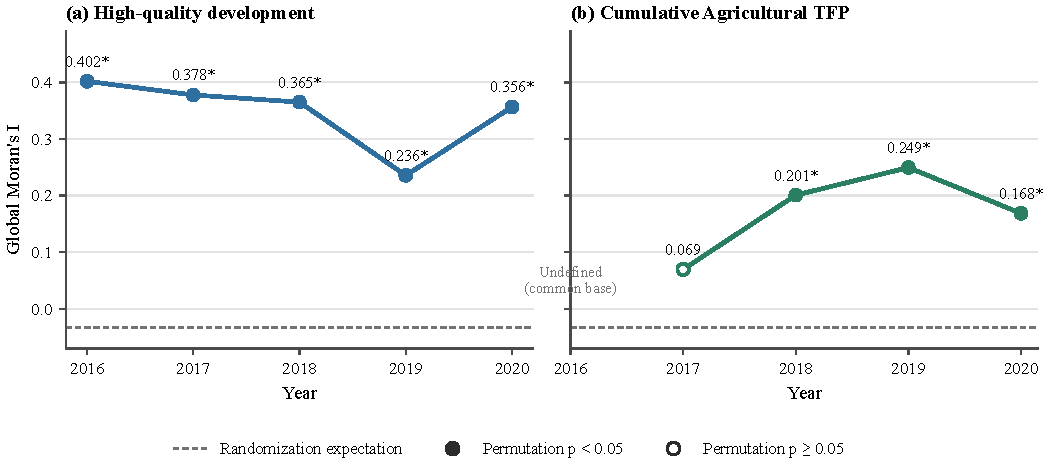
\includegraphics[width=0.96\textwidth]{figures/Figure02_Global_Moran_I.pdf}
\caption{Global spatial autocorrelation, 2016--2020. Filled markers denote permutation significance at the 5\% level; the dashed line is the randomization expectation.}
\label{fig:globalmoran}
\end{figure}

Table~\ref{tab:moran} and Figure~\ref{fig:globalmoran} show that high-quality development has a positive and significant global Moran's I in every sample year. The values are 0.402, 0.378, 0.365, 0.236, and 0.356 from 2016 to 2020, with permutation $p$ values of 0.001, 0.001, 0.003, 0.019, and 0.004, respectively. Thus, under the stated permutation convention, high values tend to be adjacent to high values and low values to low values. The index is not randomly arranged across provinces. The point estimates decline from 2016 to 2019 and recover in 2020, so the appropriate conclusion is persistent positive spatial association with annual variation rather than monotonic strengthening. No test of year-to-year differences is performed.

The global Moran's I for cumulative Agricultural TFP is undefined in 2016 because all provinces share the common base value of one, leaving no cross-sectional variance. It is 0.069 ($p=0.189$) in 2017, 0.201 ($p=0.030$) in 2018, 0.249 ($p=0.020$) in 2019, and 0.168 ($p=0.041$) in 2020. Under the source permutation convention, significance is obtained from 2018 onward, but the point estimate peaks in 2019 and falls in 2020. The 2019 TFP statistic is also slightly larger than the 2019 high-quality-development statistic (0.249 versus 0.236), so TFP association is not uniformly weaker. Because cumulative TFP measures each province's change relative to its own 2016 base, these statistics describe spatial association in cumulative growth, not spatial clustering of absolute productivity levels.

\subsubsection{Local Moran results for high-quality development}

\begin{figure}[H]
\centering
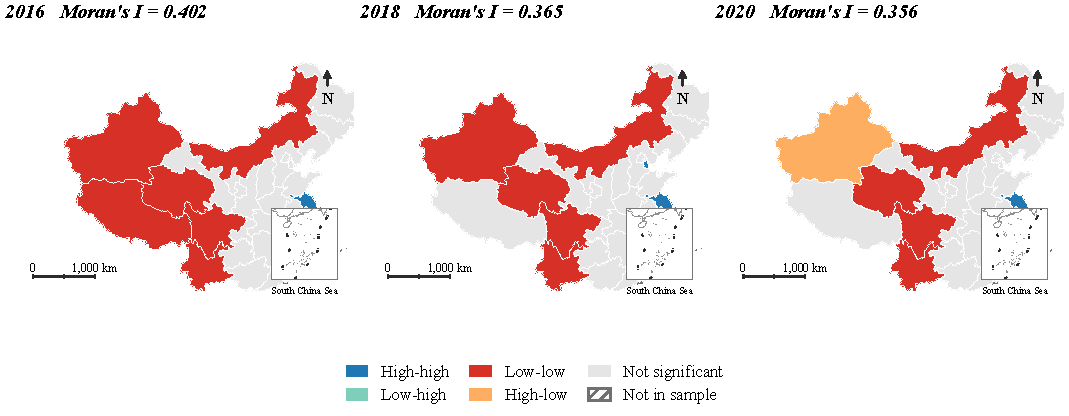
\includegraphics[width=0.96\textwidth]{figures/Figure03_Local_Moran_QDI.pdf}
\caption{Local Moran cluster maps for high-quality economic development. Cluster labels are assigned only when the local permutation test satisfies $p<0.05$; all other sampled provinces are classified as not significant.}
\label{fig:lisaqdi}
\end{figure}

\begin{figure}[H]
\centering
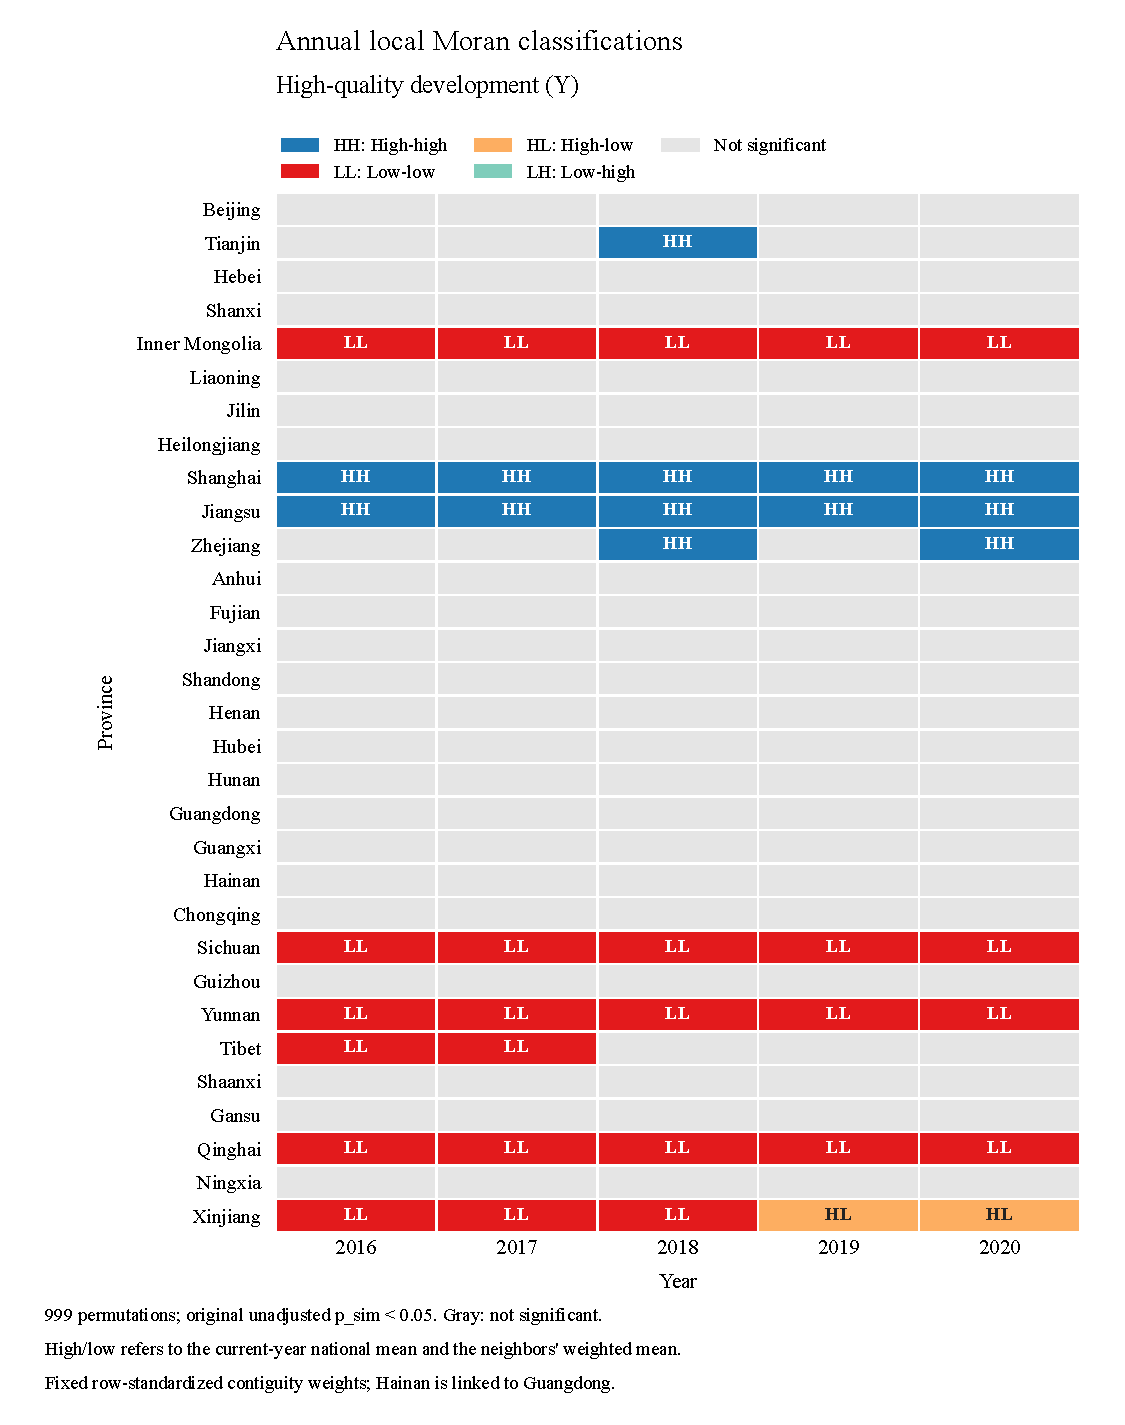
\includegraphics[width=0.78\textwidth]{figures/Moran_Annual_LISA_QDI_English.pdf}
\caption{Annual local Moran classifications for high-quality development. HH and LL denote significant high--high and low--low associations; HL and LH denote significant spatial outliers. Gray cells are not significant under the unadjusted local permutation test.}
\label{fig:lisaqdiannual}
\end{figure}

\begin{figure}[H]
\centering
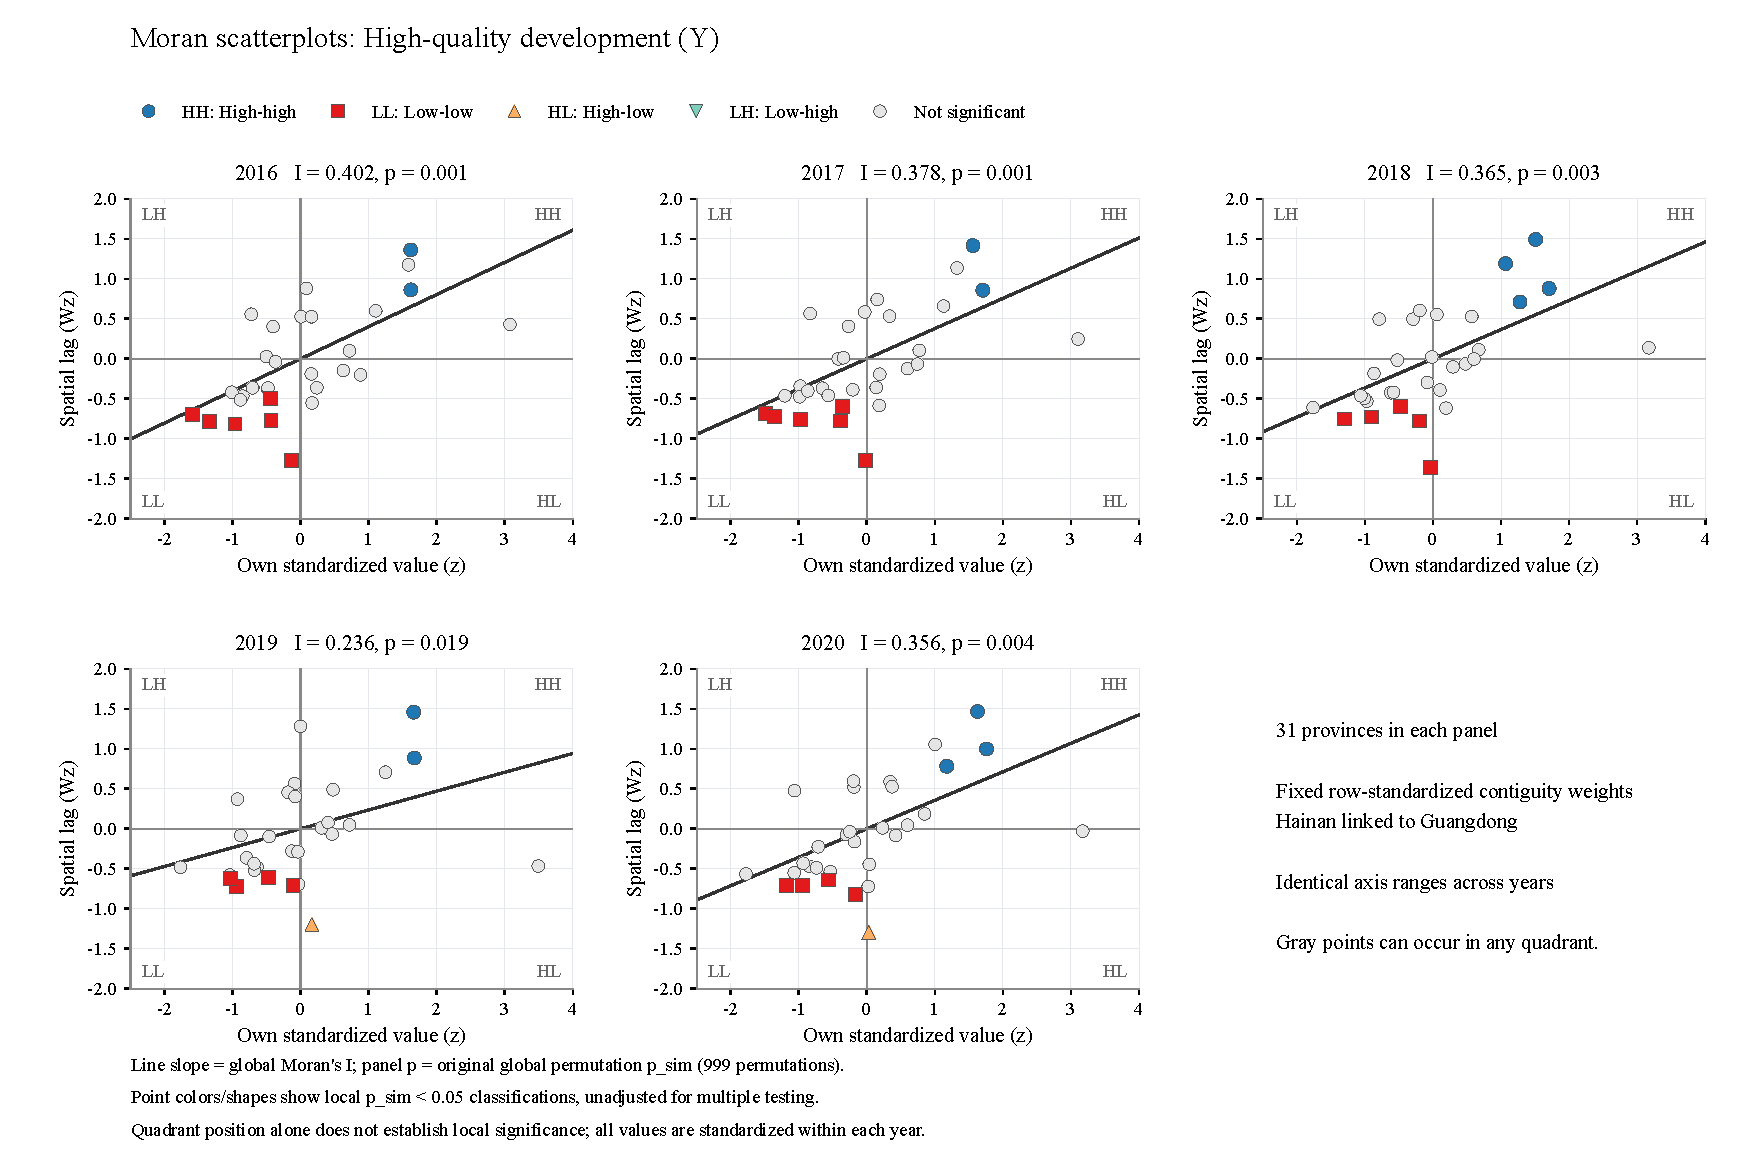
\includegraphics[width=0.96\textwidth]{figures/Moran_Scatter_QDI_English.pdf}
\caption{Moran scatterplots for high-quality development. The line slope equals the global Moran's I in each year. Point classifications use the local permutation results and are not adjusted for multiple testing.}
\label{fig:moranscatterqdi}
\end{figure}

Figures~\ref{fig:lisaqdi}--\ref{fig:moranscatterqdi} show a persistent local structure for high-quality development. In 2016 and 2017, Shanghai and Jiangsu are significant HH provinces, while Inner Mongolia, Sichuan, Yunnan, Tibet, Qinghai, and Xinjiang are significant LL provinces. In 2018, the HH set expands to Tianjin, Shanghai, Jiangsu, and Zhejiang, and the LL set contains Inner Mongolia, Sichuan, Yunnan, Qinghai, and Xinjiang. In 2019, Shanghai and Jiangsu remain HH, Inner Mongolia, Sichuan, Yunnan, and Qinghai remain LL, and Xinjiang becomes HL. In 2020, Shanghai, Jiangsu, and Zhejiang are HH, Inner Mongolia, Sichuan, Yunnan, and Qinghai are LL, and Xinjiang remains HL.

The clearest persistence is observed for Shanghai and Jiangsu, which are HH in all five years, and for Inner Mongolia, Sichuan, Yunnan, and Qinghai, which are LL in all five years. Tianjin is HH only in 2018, Zhejiang is HH in 2018 and 2020, and Tibet is LL in 2016--2017 but not significant thereafter. By year, the significant local classifications are HH=2 and LL=6 in 2016; HH=2 and LL=6 in 2017; HH=4 and LL=5 in 2018; HH=2, LL=4, and HL=1 in 2019; and HH=3, LL=4, and HL=1 in 2020. Thus, the total numbers of significant local associations are 8, 8, 9, 7, and 8. Xinjiang's transition from LL to HL indicates that its own value moved from below to slightly above the current-year national mean while its neighbors' weighted value remained below that mean. HL is a spatial-outlier category and does not imply that Xinjiang became an absolute high-development center.

\subsubsection{Local Moran results for cumulative Agricultural TFP}

\begin{figure}[H]
\centering
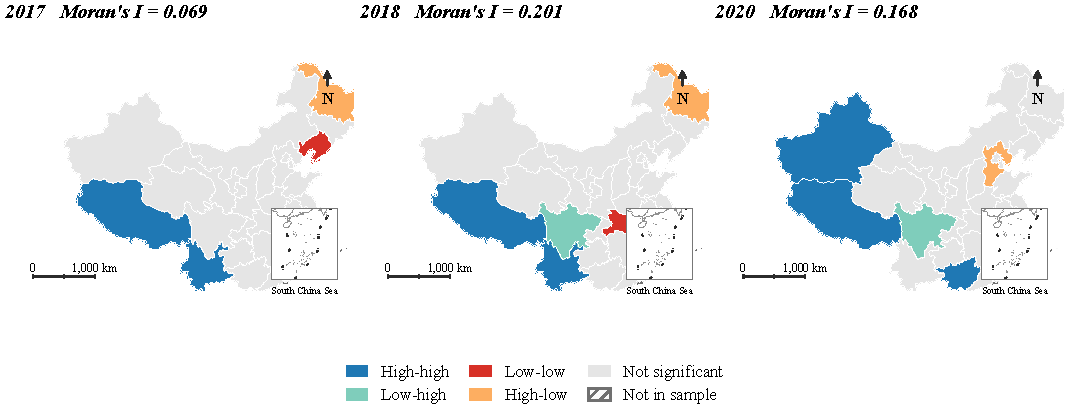
\includegraphics[width=0.96\textwidth]{figures/Figure04_Local_Moran_TFP.pdf}
\caption{Local Moran cluster maps for cumulative Agricultural TFP. The common-base year 2016 is omitted because its cross-sectional variance is zero. Cluster labels use $p<0.05$.}
\label{fig:lisatfp}
\end{figure}

\begin{figure}[H]
\centering
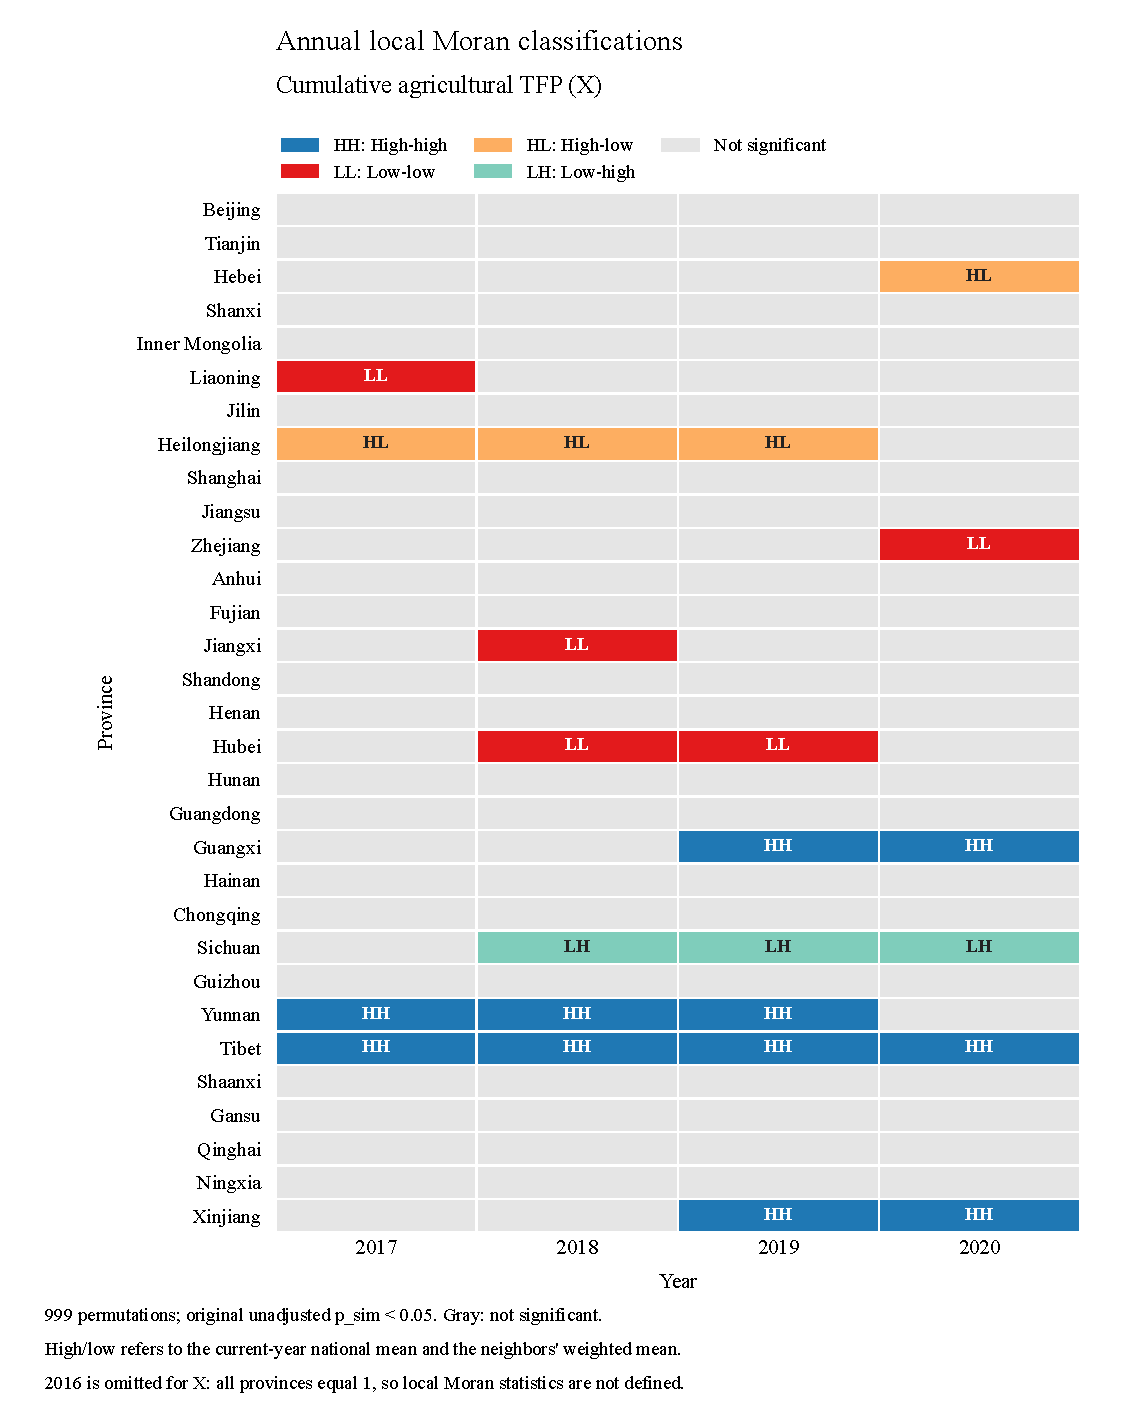
\includegraphics[width=0.78\textwidth]{figures/Moran_Annual_LISA_TFP_English.pdf}
\caption{Annual local Moran classifications for cumulative Agricultural TFP. The 2016 common-base year is omitted because all provinces equal one and local Moran statistics are undefined.}
\label{fig:lisatfpannual}
\end{figure}

\begin{figure}[H]
\centering
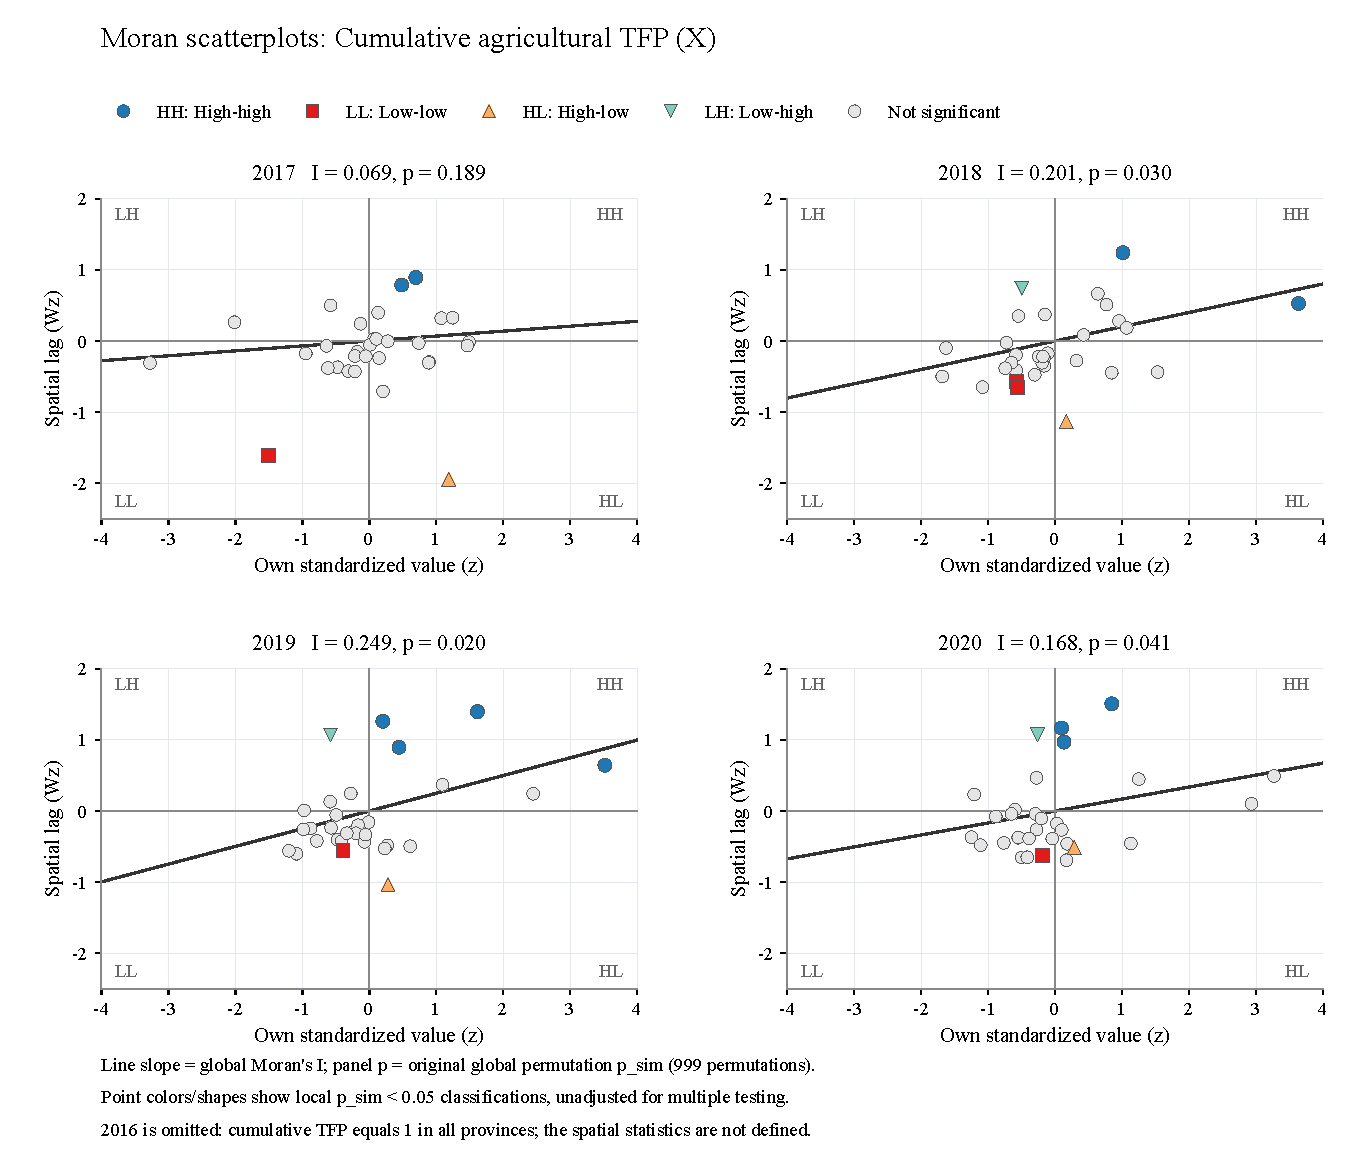
\includegraphics[width=0.96\textwidth]{figures/Moran_Scatter_TFP_English.pdf}
\caption{Moran scatterplots for cumulative Agricultural TFP. The line slope equals the global Moran's I in each year; 2016 is omitted because cumulative TFP has zero cross-sectional variance.}
\label{fig:moranscattertfp}
\end{figure}

Figures~\ref{fig:lisatfp}--\ref{fig:moranscattertfp} show less stable local clustering for cumulative Agricultural TFP. In 2017, Yunnan and Tibet are HH, Heilongjiang is HL, and Liaoning is LL. In 2018, Yunnan and Tibet remain HH, Heilongjiang remains HL, Sichuan is LH, and Jiangxi and Hubei are LL. In 2019, Guangxi, Yunnan, Tibet, and Xinjiang are HH, Heilongjiang is HL, Sichuan is LH, and Hubei is LL. In 2020, Guangxi, Tibet, and Xinjiang are HH, Hebei is HL, Sichuan is LH, and Zhejiang is LL.

Tibet is the only province that remains a significant HH location throughout 2017--2020. Yunnan is significant HH in 2017--2019, whereas Guangxi and Xinjiang become HH in 2019--2020. Heilongjiang is HL in 2017--2019 and Hebei is HL in 2020, while Sichuan is LH in 2018--2020. By year, the significant local classifications are HH=2, LL=1, and HL=1 in 2017; HH=2, LL=2, HL=1, and LH=1 in 2018; HH=4, LL=1, HL=1, and LH=1 in 2019; and HH=3, LL=1, HL=1, and LH=1 in 2020. The corresponding totals are 4, 6, 7, and 6. The nonsignificant global result in 2017 does not contradict these local findings because global and local Moran tests answer different questions. In 2020, Yunnan remains in the HH quadrant ($z=3.269$, $Wz=0.492$) but has local $p=0.091$; it is therefore classified as not significant, not as a low-growth province or as evidence that its HH quadrant position disappeared.

\subsubsection{Synthesis and transition to coupling coordination}

Taken together, high-quality development has persistent positive global spatial association and relatively stable local clusters, whereas cumulative Agricultural TFP obtains statistically significant global association from 2018 onward and exhibits more episodic local classifications. The two indicators do not share an identical spatial configuration: Yunnan is LL for high-quality development but HH for cumulative TFP in 2017--2019, while Sichuan is persistently LL for high-quality development but LH for cumulative TFP in 2018--2020. Thus, cumulative productivity growth relative to each province's own base year does not necessarily coincide with high-quality-development clustering.

These findings complement the Dagum decomposition. Dagum Gini coefficients describe the magnitude and composition of interprovincial gaps, whereas Moran statistics describe the geographic ordering of high and low observations. A narrowing Gini coefficient can therefore coexist with persistent spatial clustering, and a widening cumulative-TFP Gini coefficient need not imply a monotonic increase in Moran's I. The two approaches describe different dimensions of regional inequality and do not by themselves identify causal spillovers.

Moran's I and LISA examine the spatial dependence of each indicator separately. They do not establish whether Agricultural TFP and high-quality development are synchronized within a province, mutually reinforcing, or coordinated. Separate positive spatial autocorrelation in the two indicators does not imply that the two systems have already achieved a high level of coordination. The next section therefore applies a coupling-coordination model to quantify the relative coordination state and its evolution between Agricultural TFP and high-quality economic development under the stated normalization and weighting rules. This analysis describes joint development patterns; it does not identify causal interaction or transmission mechanisms.

\FloatBarrier
\subsection{Coupling coordination results}

\begin{table}[H]
\centering
\caption{National coupling coordination results}
\label{tab:ccdannual}
\small
\begin{tabular}{ccccccc}
\toprule
Year & Mean $U_1$ & Mean $U_2$ & Mean $C$ & Mean $T$ & Mean $D$ & Range of $D$ \\
\midrule
2016 & 0.180 & 0.365 & 0.938 & 0.273 & 0.499 & 0.393--0.619 \\
2017 & 0.181 & 0.394 & 0.900 & 0.288 & 0.504 & 0.237--0.631 \\
2018 & 0.256 & 0.414 & 0.935 & 0.335 & 0.556 & 0.411--0.677 \\
2019 & 0.351 & 0.440 & 0.961 & 0.396 & 0.614 & 0.507--0.718 \\
2020 & 0.450 & 0.462 & 0.969 & 0.456 & 0.662 & 0.578--0.767 \\
\bottomrule
\end{tabular}
\end{table}

\begin{figure}[H]
\centering
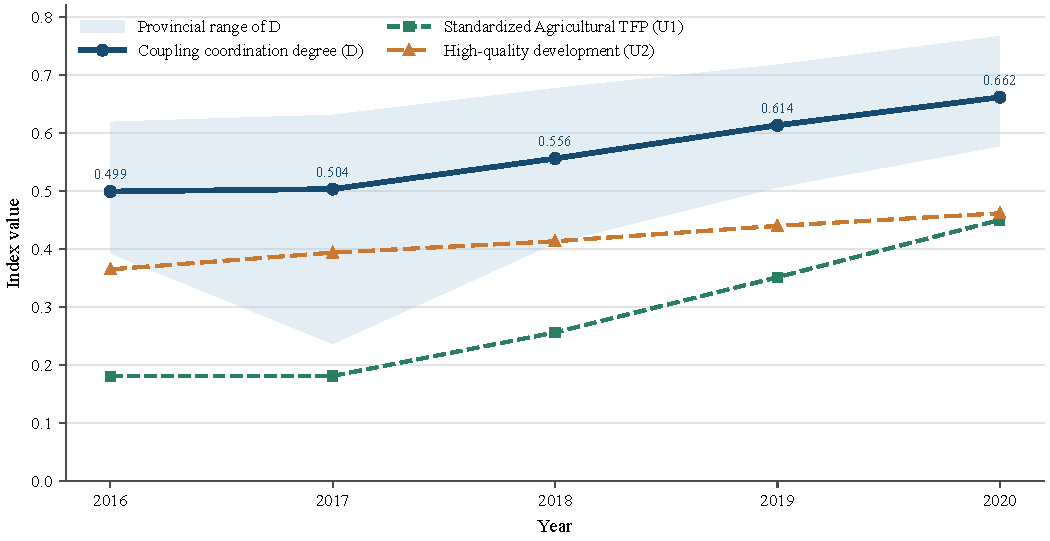
\includegraphics[width=0.90\textwidth]{figures/Figure05_Coupling_coordination_trend.pdf}
\caption{Evolution of the two subsystems and their coupling coordination degree. The shaded band gives the annual provincial range of the coupling coordination degree.}
\label{fig:ccdtrend}
\end{figure}

\begin{figure}[H]
\centering
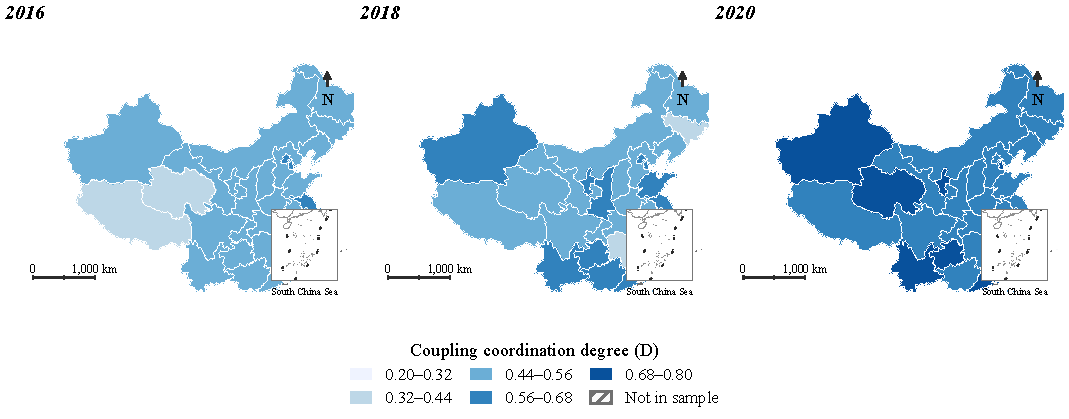
\includegraphics[width=0.98\textwidth]{figures/Figure06_Coupling_coordination_maps.pdf}
\caption{Provincial coupling coordination patterns in 2016, 2018, and 2020. Fixed bins are used across panels; Hong Kong, Macao, and Taiwan are retained on the map as not in sample.}
\label{fig:ccdmaps}
\end{figure}

\begin{table}[H]
\centering
\caption{Regional mean coupling coordination degree}
\label{tab:ccdregional}
\small
\begin{tabular}{cccc}
\toprule
Year & Eastern China & Central China & Western China \\
\midrule
2016 & 0.544 & 0.487 & 0.467 \\
2017 & 0.542 & 0.460 & 0.498 \\
2018 & 0.591 & 0.507 & 0.557 \\
2019 & 0.633 & 0.577 & 0.621 \\
2020 & 0.668 & 0.641 & 0.671 \\
\bottomrule
\end{tabular}
\end{table}

\begin{table}[H]
\centering
\caption{Provincial distribution across observed coupling coordination levels}
\label{tab:ccdlevels}
\footnotesize
\begin{tabular}{c rrrrrr}
\toprule
Year & \shortstack{Mild\\disequilibrium} & \shortstack{Moderate\\disequilibrium} & \shortstack{Near\\disequilibrium} & \shortstack{Barely\\coordinated} & \shortstack{Primary\\coordination} & \shortstack{Intermediate\\coordination} \\
\midrule
2016 & 1 & 0 & 16 & 13 & 1 & 0 \\
2017 & 0 & 1 & 12 & 16 & 2 & 0 \\
2018 & 0 & 0 & 3 & 22 & 6 & 0 \\
2019 & 0 & 0 & 0 & 14 & 14 & 3 \\
2020 & 0 & 0 & 0 & 2 & 23 & 6 \\
\bottomrule
\end{tabular}
\parbox{0.94\textwidth}{\footnotesize\textit{Note:} The table reports the nonzero categories observed in the sample; extreme disequilibrium, severe disequilibrium, good coordination, and excellent coordination have zero observations in every year.}
\end{table}

\begin{table}[H]
\centering
\caption{Sensitivity of coupling coordination results}
\label{tab:ccdsensitivity}
\footnotesize
\begin{threeparttable}
\begin{tabular}{lccc}
\toprule
Specification & Mean $D$, 2016 & Mean $D$, 2020 & \shortstack{Rank correlation\\with baseline} \\
\midrule
Baseline: full-sample min--max & 0.499 & 0.662 & 1.000 \\
No zero shift & 0.494 & 0.660 & 1.000 \\
Winsorized min--max & 0.463 & 0.663 & 0.991 \\
Percentile rank & 0.522 & 0.779 & 0.941 \\
TFP weight 0.4 & 0.515 & 0.663 & 0.986 \\
TFP weight 0.6 & 0.484 & 0.661 & 0.989 \\
Year-specific min--max & 0.646 & 0.561 & 0.020 \\
\bottomrule
\end{tabular}
\begin{tablenotes}[flushleft]\footnotesize
\item Notes: Rank correlations use all 155 province--year observations. Year-specific min--max scaling removes intertemporal level comparability and is included as a diagnostic rather than a preferred specification.
\end{tablenotes}
\end{threeparttable}
\end{table}

Tables~\ref{tab:ccdannual}--\ref{tab:ccdlevels}, Figures~\ref{fig:ccdtrend}--\ref{fig:ccdmaps},
and the sensitivity results in Table~\ref{tab:ccdsensitivity} show that the mean
coupling degree $C$ between Agricultural TFP and high-quality economic
development remained high throughout the sample (0.900--0.969), whereas the
mean coupling coordination degree $D$ improved gradually from a relatively low
level. This pattern indicates that the two subsystems were broadly matched in
relative terms. The relatively low early values of $D$ were therefore mainly
constrained by the insufficient joint level of the two subsystems, rather than
by a fundamental coordination barrier between them. Because $C$ primarily
captures relative balance, two systems can obtain a high $C$ even when both are
at relatively low levels, provided that their development levels are close. The
comprehensive index $T$, by contrast, reflects the overall level of both systems
and consequently constrains $D$.

Between 2016 and 2017, mean $D$ increased only slightly, from 0.499 to 0.504,
while mean $T$ rose from 0.273 to 0.288, indicating that the two systems were
still at a relatively low stage of joint development. The coupling degree fell
to its sample minimum of 0.900 in 2017, suggesting some fluctuation in relative
matching. After 2018, mean standardized Agricultural TFP $U_1$ increased from
0.256 to 0.450 and $T$ rose from 0.335 to 0.456, pushing $D$ to 0.662 by 2020.
The improvement in coordination therefore primarily reflects the joint
strengthening of the two subsystems and a more favorable balance between them.

The level distribution in Table~\ref{tab:ccdlevels} confirms a broad upward
transition. In 2016, 16 provinces were near disequilibrium and 13 were barely
coordinated, with one province in mild disequilibrium and one in primary
coordination. In 2017, one province was moderately disequilibrated, while the
barely coordinated and primary-coordination groups increased to 16 and 2,
respectively. In 2018, 22 provinces were barely coordinated and 6 reached
primary coordination. In 2019, 14 provinces were barely coordinated, 14 were in
primary coordination, and 3 reached intermediate coordination. By 2020, 23
provinces were in primary coordination and 6 in intermediate coordination, with
only 2 remaining barely coordinated. No province reached good or excellent
coordination, so the improvement represents a shift from the edge of
disequilibrium toward primary and intermediate coordination rather than a
transition to the highest coordination levels.

The regional means in Table~\ref{tab:ccdregional} reveal substantial
heterogeneity. Eastern China led in 2016 ($D=0.544$) and reached 0.668 in 2020;
central China rose from 0.487 to 0.641; and western China increased from 0.467
to 0.671, the largest gain, narrowly exceeding the east at the end of the
sample. This result does not imply that western China overtook the east in
absolute high-quality development. Rather, the western increase primarily
reflects rapid cumulative TFP growth and the associated rise in standardized
$U_1$, whereas eastern China retained the higher high-quality-development
subsystem level. Regional $D$ therefore measures the balance of the two
standardized subsystems, not a ranking of high-quality development alone.

The post-2017 improvement may also be viewed in the institutional context of
the formal policy emphasis placed on high-quality development after 2017. That
shift may have strengthened local attention to development quality, efficiency,
and structural transformation. However, total factor productivity was not
introduced in 2017; its theoretical foundations and agricultural applications
predate the sample period. The increase in $D$ after 2018 therefore cannot be
attributed directly to that policy milestone. Moreover, cumulative Agricultural
TFP is defined relative to a common 2016 base and standardized over the full
sample, so the relatively low early values of $U_1$, $T$, and $D$ also contain a
mechanical component arising from the base-year and normalization choices.

The near-unity rank correlations under the zero-shift, winsorized, and
alternative-weight specifications in Table~\ref{tab:ccdsensitivity} show that
the upward movement and broad provincial ordering are not driven by a single
minor modeling choice. The percentile transformation changes the absolute
level but preserves the overall increase. In contrast, year-specific scaling
discards common time movement and produces a very different ordering, so it is
not suitable for the main intertemporal interpretation.

Overall, the evidence is more consistent with a level constraint than with an
inability of Agricultural TFP and high-quality development to coordinate. The
early low coordination degree mainly reflects the modest joint level of the two
subsystems, together with the construction of cumulative TFP from a common base
year. The post-2017 policy environment may provide relevant institutional
context, but its specific contribution requires a longer panel and a dedicated
policy-identification strategy.

Taken together, the kernel-density estimates, Dagum Gini decomposition, Moran's
$I$ statistics, and coupling-coordination analysis establish four complementary
descriptive facts. The high-quality economic development index shifted upward
and became less dispersed across provinces, whereas cumulative Agricultural TFP
increased but became more regionally differentiated. Both indicators exhibited
spatial dependence, although their local clustering patterns were not identical.
Their joint coordination improved overall, but the average degree remained
mainly within the primary- to intermediate-coordination range.

These analyses respectively describe how the distributions changed, where
disparities originated, whether spatial clustering existed, and whether the two
systems evolved jointly. They remain, however, unconditional descriptive
evidence. They do not determine whether Agricultural TFP is systematically
associated with high-quality economic development after accounting for other
factors, nor do they eliminate the possible influence of time-invariant
provincial characteristics and common time shocks. The next section therefore
employs a two-way fixed-effects model with province and year effects. Controlling
for population density, industrial structure, and the other specified
covariates, this model tests the conditional association between Agricultural
TFP and high-quality economic development. Given the short panel and the
possibility of reverse causality, the estimated coefficient should be
interpreted as a conditional statistical association rather than as a causal
effect.

\FloatBarrier
\subsection{Baseline, robustness, and endogeneity checks}

\subsubsection{Baseline specification and results}

Table~\ref{tab:baseline} reports five nested specifications of
Equation~\ref{eq:fe}. Column (1) regresses $\ln Y$ on $\ln TFP$ alone;
column (2) adds population density and the primary-sector share.
Columns (3) and (4) additionally include year and province effects,
respectively, and column (5) includes both sets of effects.
This sequence separates the roles of observed controls, common time
shocks, and persistent provincial heterogeneity.

\begin{table}[H]
\centering
\begin{threeparttable}
\caption{Baseline regressions of high-quality economic development on cumulative agricultural TFP}
\label{tab:baseline}
\footnotesize
\begin{tabularx}{\textwidth}{l*{5}{>{\centering\arraybackslash}X}}
\toprule
Dependent variable: $\ln Y$ & (1) & (2) & (3) & (4) & (5) \\
& OLS & OLS & Year FE & Province FE & Two-way FE \\
\midrule
$\ln TFP$ & $-0.019$ & $0.293$\sym{**} & $-0.279$\sym{*} & $0.716$\sym{***} & $0.446$\sym{**} \\
& (0.134) & (0.107) & (0.163) & (0.118) & (0.194) \\
& [$-0.145$] & [2.723] & [$-1.714$] & [6.090] & [2.300] \\
\addlinespace
$\ln$ population density & -- & $0.140$\sym{***} & $0.128$\sym{***} & $-0.644$ & $-0.104$ \\
& & (0.030) & (0.027) & (1.274) & (1.342) \\
& & [4.726] & [4.702] & [$-0.505$] & [$-0.077$] \\
\addlinespace
Primary-sector share & -- & $-0.017$\sym{**} & $-0.016$\sym{**} & $-0.040$\sym{**} & $-0.003$ \\
& & (0.007) & (0.006) & (0.018) & (0.026) \\
& & [$-2.405$] & [$-2.545$] & [$-2.293$] & [$-0.111$] \\
\midrule
Controls & No & Yes & Yes & Yes & Yes \\
Province effects & No & No & No & Yes & Yes \\
Year effects & No & No & Yes & No & Yes \\
Observations & 155 & 155 & 155 & 155 & 155 \\
Provinces & 31 & 31 & 31 & 31 & 31 \\
$R^2$ & 0.000 & 0.591 & 0.662 & 0.948 & 0.957 \\
Adjusted $R^2$ & $-0.006$ & 0.583 & 0.646 & 0.934 & 0.943 \\
\bottomrule
\end{tabularx}
\begin{tablenotes}[flushleft]
\footnotesize
\item Notes: Province-clustered CR1 standard errors are in parentheses;
$t$ statistics are in brackets. Tests use $t_{30}$.
\sym{***}$p<0.01$, \sym{**}$p<0.05$, \sym{*}$p<0.10$.
The primary-sector share is measured in percentage points.
Intercepts and fixed-effect coefficients are omitted. $R^2$ and adjusted
$R^2$ refer to the full dummy-variable regressions, including fixed effects,
and are not within-$R^2$ measures.
\end{tablenotes}
\end{threeparttable}
\end{table}


The unconditional association in column (1) is close to zero and statistically
indistinguishable from zero ($\hat\beta=-0.019$, $p=0.885$; 95\% confidence
interval $[-0.292,0.253]$). Adding the controls changes the
estimate to 0.293 ($p=0.011$), and raises adjusted
$R^2$ from $-0.006$ to 0.583. The estimate becomes negative when only year
effects are added ($-0.279$, $p=0.097$), but is positive and precisely
estimated when province effects are included ($0.716$, $p<0.001$).
The sign reversal across specifications highlights sensitivity to the
treatment of provincial heterogeneity. It motivates conditioning on
province effects but does not, by itself, identify a causal effect or the
direction of omitted-variable bias.

The preferred two-way fixed-effects estimate in column (5) is 0.446
(province-clustered standard error 0.194, $p=0.029$).
A 1\% increase in cumulative agricultural TFP is therefore associated
with an approximately 0.446\% increase in the high-quality development
index, conditional on the controls and both sets of fixed effects.
The 95\% confidence interval is [0.050, 0.842]. Population density and
the primary-sector share are not statistically significant in this
specification. Adjusted $R^2$ is 0.943 when the fixed-effect indicators
are included in the fitted model; this should not be confused with the
within-$R^2$ of 0.526 reported below.
The estimate supports the positive conditional association in H1.
Reverse causality and time-varying omitted factors nevertheless preclude
a causal interpretation of this coefficient alone.

\subsubsection{Robustness and endogeneity}

Table~\ref{tab:robustness} summarizes the alternative specifications using
the same province-clustered CR1 correction and $t_{G-1}$ inference whenever
clustering is used. The accompanying forest plot places the estimates on a
common elasticity scale; the levels specification is reported in the table
but omitted from the plot because it uses a different scale.

\begin{table}[H]
\centering
\begin{threeparttable}
\caption{Baseline and robustness estimates for Agricultural TFP}
\label{tab:robustness}
\footnotesize
\begin{tabular}{lccccc}
\toprule
Specification & Coefficient & Std. error & $p$-value & $N$ & Within $R^2$ \\
\midrule
Baseline two-way FE & 0.446\sym{**} & 0.194 & 0.029 & 155 & 0.526 \\
Winsorized at 1\% & 0.382\sym{**} & 0.149 & 0.016 & 155 & 0.502 \\
Excluding municipalities & 0.493\sym{**} & 0.204 & 0.023 & 135 & 0.586 \\
Lagged Agricultural TFP & 0.255 & 0.154 & 0.109 & 124 & 0.348 \\
Levels specification & 0.043 & 0.030 & 0.160 & 155 & 0.258 \\
Driscoll--Kraay standard errors & 0.446\sym{***} & 0.091 & $<0.001$ & 155 & 0.526 \\
\bottomrule
\end{tabular}
\begin{tablenotes}[flushleft]
\footnotesize
\item Notes: \sym{***}$p<0.01$, \sym{**}$p<0.05$, \sym{*}$p<0.10$.
All models include province and year effects and the two controls.
Clustered specifications use CR1 standard errors and $t_{G-1}$ inference
($G=31$, or 27 when municipalities are excluded).
The Driscoll--Kraay row uses a Bartlett kernel, bandwidth two, and
$t_{117}$ inference. Within $R^2$ excludes the fit attributed to
province effects.
\end{tablenotes}
\end{threeparttable}
\end{table}

\begin{figure}[H]
\centering
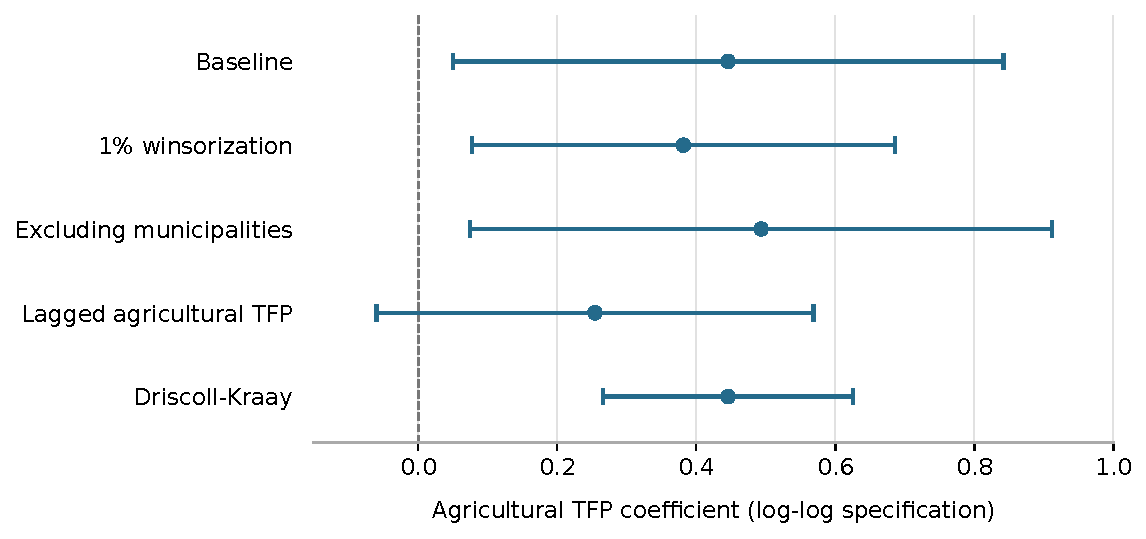
\includegraphics[width=\textwidth]{figure1/Robustness_forest_CR1_English.pdf}
\caption{Robustness of the agricultural TFP coefficient. Points are elasticity estimates and bars are 95\% confidence intervals using the covariance corrections and reference distributions stated in Table~\ref{tab:robustness}. The levels specification is excluded because it is on a different coefficient scale.}
\label{fig:robustness}
\end{figure}

Across the alternative specifications, the coefficient remains positive and
statistically significant after one-percent winsorization and after excluding
the four municipalities. The lagged estimate remains positive but is not
significant at the 10\% level ($p=0.109$), and the levels specification is also
insignificant ($p=0.160$). The direction is therefore stable, whereas
statistical significance is not uniform. The winsorization and municipality
exclusion checks address influential observations and sample composition; the
lagged specification reduces contemporaneous simultaneity; the levels model
tests functional-form sensitivity; and the Driscoll--Kraay correction provides
a separate covariance check for cross-sectional and serial dependence. The
Driscoll--Kraay result is more precise, but with only five annual observations
it remains a sensitivity check rather than decisive evidence about the error
dependence structure.

Table~\ref{tab:iv} reports a same-sample comparison between two-way
fixed-effects OLS and an internal-instrument 2SLS specification. The
first-stage strength and Wu--Hausman diagnostics are reported alongside the
second-stage estimate.

\begin{table}[H]
\centering
\caption{Internal-instrument endogeneity check}
\label{tab:iv}
\footnotesize
\begin{tabularx}{\textwidth}{Xccccc}
\toprule
Model & Coefficient & Standard error & $p$-value & \shortstack{First-stage\\partial $F$} & Observations \\
\midrule
Same-sample fixed-effects OLS & 0.396\sym{***} & 0.145 & 0.008 & -- & 124 \\
2SLS with lagged TFP & 0.526\sym{*} & 0.271 & 0.055 & 39.36 & 124 \\
\bottomrule
\end{tabularx}
\end{table}

The same-sample fixed-effects OLS estimate is 0.396 ($p=0.008$), whereas
using one-period lagged Agricultural TFP as an internal instrument gives a
2SLS estimate of 0.526 ($p=0.055$; 95\% confidence interval approximately
$[-0.012,1.064]$). The first-stage partial $F$ statistic is 39.36, providing
no indication of a weak-instrument problem under the usual rule of thumb.
The Wu--Hausman test does not reject exogeneity ($p=0.401$), so the difference
between the two estimates is not statistically decisive. Because the
instrument is internally generated, its exclusion restriction cannot be
verified, and the panel has only four usable transition years. This check
therefore supports the sign of the conditional association but does not
establish strict causality.

\FloatBarrier
\subsection{Spatial Durbin estimates and impact decomposition}

Table~\ref{tab:sdm} reports the coefficient estimates from the spatial Durbin
model. The impact decomposition in Figure~\ref{fig:spatialimpacts} then
translates these coefficients into feedback-adjusted direct, indirect, and
total effects.

\begin{table}[H]
\centering
\caption{Selected spatial Durbin model estimates}
\label{tab:sdm}
\small
\begin{tabular}{lccc}
\toprule
Variable & Coefficient & Standard error & $p$-value \\
\midrule
$\ln TFP$ & 0.355\sym{***} & 0.087 & $<0.001$ \\
$W\ln TFP$ & 0.166 & 0.183 & 0.365 \\
$\ln$ population density & $-0.762$ & 0.634 & 0.230 \\
$W\ln$ population density & 1.822\sym{*} & 1.053 & 0.083 \\
Primary-sector share & 0.004 & 0.014 & 0.779 \\
$W$ primary-sector share & 0.031 & 0.026 & 0.238 \\
Spatial autoregressive coefficient $\rho$ & 0.216\sym{**} & 0.102 & 0.035 \\
\bottomrule
\multicolumn{4}{l}{\footnotesize \sym{***}$p<0.01$, \sym{**}$p<0.05$, \sym{*}$p<0.10$. Province and year effects included.}
\end{tabular}
\end{table}

\begin{figure}[H]
\centering
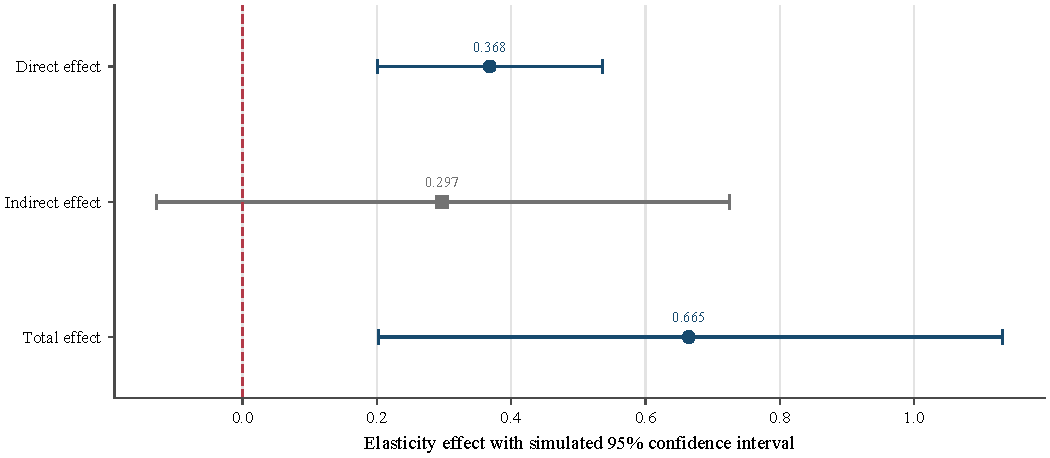
\includegraphics[width=0.78\textwidth]{figures/Figure08_Spatial_impact_decomposition.pdf}
\caption{Direct, indirect, and total effects from the spatial model. Bars are simulated 95\% confidence intervals.}
\label{fig:spatialimpacts}
\end{figure}

Table~\ref{tab:sdm} and Figure~\ref{fig:spatialimpacts} show a significant
local association but no statistically established cross-provincial
Agricultural TFP spillover. The spatial autoregressive coefficient is 0.216
($p=0.035$), indicating positive spatial dependence in high-quality
development after controls and province and year effects. The own-region
coefficient on log Agricultural TFP is 0.355 ($p<0.001$), whereas the
coefficient on spatially lagged TFP is 0.166 ($p=0.365$). The latter is not
itself the spillover effect, because spatial feedback must be incorporated
through the impact decomposition in Equation~\ref{eq:impact}.

The feedback-adjusted direct, indirect, and total effects are 0.368
($p<0.001$), 0.297 ($p=0.164$), and 0.665 ($p=0.004$), respectively. Thus,
Agricultural TFP is positively associated with high-quality development in
the own province, and the total response is statistically significant.
However, the indirect component is positive but too imprecisely estimated to
confirm a stable cross-provincial spillover; the significant total effect is
driven mainly by the direct effect.

\FloatBarrier
\subsection{Development-stage heterogeneity: threshold effect}

To examine whether the conditional association varies with the development
stage of a province, we use the logarithm of GDP per capita as the threshold
variable and estimate a single-threshold panel model. Table~\ref{tab:threshold}
reports the threshold test and regime-specific coefficients, while
Figure~\ref{fig:threshold} displays the likelihood-ratio statistic profile.

\begin{table}[H]
\centering
\caption{Single-threshold test and regime-specific Agricultural TFP coefficients}
\label{tab:threshold}
\small
\begin{tabular}{lcccc}
\toprule
Item & Estimate & Standard error & $p$-value & Observations \\
\midrule
Sup-F statistic (no threshold) & 47.646 & -- & 0.002\textsuperscript{a} & 155 \\
Threshold $\widehat\gamma$ & 11.069 & -- & -- & 155 \\
$\ln TFP$ when $q\le\widehat\gamma$ & 0.375\sym{**} & 0.171 & 0.036 & 106 \\
$\ln TFP$ when $q>\widehat\gamma$ & $-0.344$ & 0.222 & 0.133 & 49 \\
\bottomrule
\multicolumn{5}{l}{\footnotesize \textsuperscript{a} Wild cluster-bootstrap $p$-value for the no-threshold test, based on 499 replications.}
\end{tabular}
\end{table}

\begin{figure}[H]
\centering
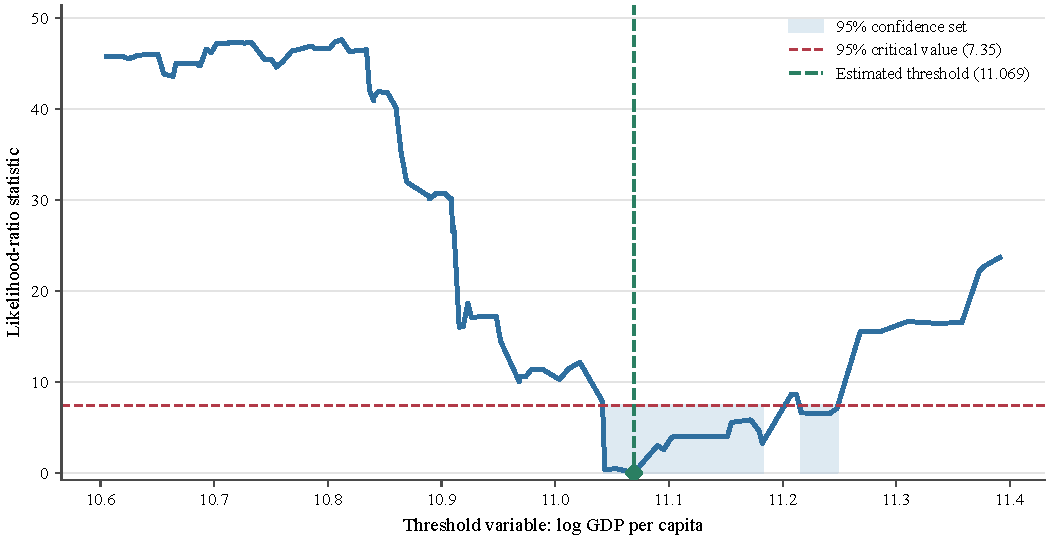
\includegraphics[width=0.82\textwidth]{figures/Figure09_Threshold_profile.pdf}
\caption{Profile of the likelihood-ratio statistic for the estimated GDP-per-capita threshold. Shaded regions denote the accepted segments of the 95\% likelihood-ratio confidence set; the red dashed line is the critical value, and the green dashed line marks the estimated threshold.}
\label{fig:threshold}
\end{figure}

Table~\ref{tab:threshold} and Figure~\ref{fig:threshold} indicate
development-stage heterogeneity in the Agricultural TFP association. The LR
profile reaches its minimum at $\widehat\gamma=11.069$, corresponding to GDP
per capita of approximately RMB 64,171. The Sup-F statistic is 47.646, and the
499-replication wild-cluster bootstrap rejects the null of no threshold
($p=0.002$). The 95\% LR confidence set consists of two accepted segments,
approximately [11.044, 11.182] and [11.216, 11.248], rather than one
continuous interval.

At or below the threshold, the log Agricultural TFP coefficient is 0.375
($p=0.036$), based on 106 province--year observations. Because the model is
specified in logarithms, a 1\% increase in Agricultural TFP is associated with
an approximately 0.375\% increase in the high-quality development index in
this regime. Above the threshold, the coefficient is $-0.344$ ($p=0.133$),
based on 49 observations. It is statistically indistinguishable from zero;
therefore, the result indicates attenuation and loss of significance rather
than evidence that Agricultural TFP harms high-quality development at higher
income levels.

The pattern is consistent with stronger productivity leverage where resource
and income constraints are binding and relatively lower marginal relevance at
higher development stages, when innovation, modern services, human capital,
and public governance may become more important. This is a mechanism
interpretation rather than a causal identification. Moreover, GDP per capita
(PCGDP) is one of the 16 indicators entering $Y$, so the threshold result
should be read as an index-specific development-stage pattern, not as a
universal causal cutoff. A leave-one-out index or a lagged GDP-per-capita
threshold would provide a useful additional sensitivity check in a longer
panel.

\FloatBarrier
\subsection{Spatial Markov transitions}

Table~\ref{tab:spatial_markov} reports the unconditional and
neighborhood-conditioned transition probabilities for high-quality
development. The construction of the states and neighborhood contexts is
defined in the table notes.

\begin{table}[H]
\caption{Spatially Conditioned Markov Transition Probabilities for High-Quality Economic Development\label{tab:spatial_markov}}
\small
\begin{tabularx}{\textwidth}{llr>{\centering\arraybackslash}X>{\centering\arraybackslash}X>{\centering\arraybackslash}X>{\centering\arraybackslash}X}
\toprule
\textbf{Neighborhood context} & \textbf{Current state} & \textbf{$N$} & \multicolumn{4}{c}{\textbf{Next-period state}} \\
\cmidrule(lr){4-7}
 & & & \textbf{Low} & \textbf{Lower-middle} & \textbf{Upper-middle} & \textbf{High} \\
\midrule
\multirow{4}{*}{Unconditional} & Low & 32 & 0.969 & 0.031 & 0.000 & 0.000 \\
 & Lower-middle & 32 & 0.031 & 0.844 & 0.125 & 0.000 \\
 & Upper-middle & 28 & 0.000 & 0.107 & 0.750 & 0.143 \\
 & High & 32 & 0.000 & 0.031 & 0.094 & 0.875 \\
\midrule
\multirow{4}{*}{Low-neighbor} & Low & 22 & 1.000 & 0.000 & 0.000 & 0.000 \\
 & Lower-middle & 13 & 0.077 & 0.846 & 0.077 & 0.000 \\
 & Upper-middle & 8 & 0.000 & 0.000 & 1.000 & 0.000 \\
 & High & 1 & 0.000 & 0.000 & 0.000 & 1.000 \\
\midrule
\multirow{4}{*}{Middle-neighbor} & Low & 6 & 0.833 & 0.167 & 0.000 & 0.000 \\
 & Lower-middle & 13 & 0.000 & 0.923 & 0.077 & 0.000 \\
 & Upper-middle & 11 & 0.000 & 0.000 & 0.818 & 0.182 \\
 & High & 10 & 0.000 & 0.100 & 0.100 & 0.800 \\
\midrule
\multirow{4}{*}{High-neighbor} & Low & 4 & 1.000 & 0.000 & 0.000 & 0.000 \\
 & Lower-middle & 6 & 0.000 & 0.667 & 0.333 & 0.000 \\
 & Upper-middle & 9 & 0.000 & 0.333 & 0.444 & 0.222 \\
 & High & 21 & 0.000 & 0.000 & 0.095 & 0.905 \\
\bottomrule
\end{tabularx}
\vspace{2pt}
\noindent\footnotesize\textit{Notes:} States are annual quartiles of the high-quality development index. Neighborhood contexts are terciles of the origin-year spatial lag, so conditioning never uses future information. $N$ gives transition counts for each origin row; every nonempty probability row sums to one. Shorrocks mobility indices are Unconditional: 0.188; Low-neighbor: 0.051; Middle-neighbor: 0.208; High-neighbor: 0.328. A 999-permutation test of equality across the three conditional matrices gives $G=21.76$ and $p=0.087$.
\end{table}

The transition matrix is strongly diagonal: the probability of remaining in
the same state is 0.969 for low, 0.844 for lower-middle, 0.750 for
upper-middle, and 0.875 for high states. The unconditional Shorrocks mobility
index is 0.188. Conditional mobility is 0.051 in low-neighbor environments,
0.208 in middle-neighbor environments, and 0.328 in high-neighbor
environments. Hence, high-quality development states are persistent,
especially in low-neighbor contexts, whereas high-neighbor contexts are more
mobile. Mobility alone, however, does not identify whether transitions are
upward or downward.

The permutation test of equality across the conditional matrices gives
$G=21.76$ and $p=0.087$. Neighborhood conditioning is therefore marginally
significant at the 10\% level but not at the 5\% level. The sample does not
establish a stable neighborhood-promoting effect or a definite spatial trap.
Because only 124 one-year transitions are available, the conditional matrices
should be interpreted as descriptive transition evidence rather than as
long-run forecasts.

\section{Discussion}

The evidence yields a coherent but qualified picture. At the descriptive level, the
high-quality development index moved upward, with its mean increasing from
0.365 to 0.462 and its Dagum Gini coefficient declining from 0.215 to 0.141.
Cumulative Agricultural TFP also increased, from its common base of 1.000 to
1.386, but its Gini coefficient rose from 0.040 in 2017 to 0.085 in 2020.
The Dagum components indicate that convergence in development quality reflected
declining within- and net between-region differences, whereas the widening TFP
gap was associated mainly with a larger net between-region component and higher
within-region inequality in eastern and western China. Productivity growth and
development quality therefore followed different regional distributional paths
and should not be treated as interchangeable outcomes.

The spatial evidence supports H2 only in a qualified sense. High-quality
development has significant positive global Moran's $I$ in every year (0.402,
0.378, 0.365, 0.236, and 0.356), together with persistent eastern HH and
western or northern LL local clusters. Cumulative-TFP Moran's $I$ is undefined
in 2016 because of the common base, insignificant in 2017 ($I=0.069$,
$p=0.189$), and significant from 2018 ($I=0.201$, $p=0.030$) through 2020
($I=0.168$, $p=0.041$), with more transient local types. Positive spatial
dependence is therefore clear for development quality and emerges later for
cumulative TFP, but neither series displays a monotonic increase in clustering.
Moran statistics describe geographic ordering, not causal spillovers.

The coupling results add a level--balance distinction. Mean coupling $C$
remained high (0.900--0.969), indicating that the two standardized subsystems
were relatively well matched. Mean coupling coordination $D$ rose from 0.499
in 2016 to 0.662 in 2020, and the distribution shifted from the edge of
disequilibrium toward primary and intermediate coordination. The improvement
is mainly associated with rising subsystem levels and a better balance, rather
than with evidence of a fundamental inability to coordinate. Because cumulative
TFP is based at 2016 and standardized over the full sample, the absolute level
of $D$ is normalization-dependent. The high western $D$ in 2020 should not be
read as the west overtaking the east in the level of high-quality development.

The econometric results provide the clearest evidence for H1, but as a
conditional association. In the preferred two-way fixed-effects model, the
Agricultural TFP coefficient is 0.446 (province-clustered standard error
0.194, $p=0.029$; 95\% CI [0.050, 0.842]). The coefficient remains positive and
significant under one-percent winsorization (0.382, $p=0.016$), after
excluding municipalities (0.493, $p=0.023$), and with Driscoll--Kraay standard
errors (0.446, $p<0.001$). It remains positive but is not significant in the
lagged specification (0.255, $p=0.109$) or the levels specification (0.043,
$p=0.160$). The same-sample 2SLS estimate is 0.526 ($p=0.055$), with a
first-stage partial $F=39.36$ and a Wu--Hausman $p=0.401$; however, the internal
instrument's exclusion restriction cannot be verified. H1 is thus supported as
a positive conditional relationship, not as a causal elasticity.

H3 is only partially supported. In the spatial Durbin model, the spatial
autoregressive coefficient for development quality is positive
($\rho=0.216$, $p=0.035$), and the feedback-adjusted direct effect of
Agricultural TFP is 0.368 ($p<0.001$). The indirect effect is positive (0.297)
but not statistically distinguishable from zero ($p=0.164$); the total effect
is 0.665 ($p=0.004$), driven mainly by the direct component. The data therefore
support a local Agricultural TFP--development association and outcome-level
spatial dependence, but do not establish a stable cross-provincial productivity
spillover.

H4 receives statistical support for development-stage heterogeneity. The
threshold test rejects no threshold (Sup-$F=47.646$, wild-cluster-bootstrap
$p=0.002$) at log GDP per capita 11.069, approximately RMB 64,171. Below the
threshold, the coefficient is 0.375 ($p=0.036$); above it, the estimate is
$-0.344$ ($p=0.133$), indicating attenuation and loss of significance rather
than significant harm. A plausible interpretation is that productivity gains
relax tighter income and resource constraints in lower-development regions,
whereas innovation, services, human capital, and governance become relatively
more binding at higher stages. This remains a mechanism interpretation rather
than a causal explanation. Since GDP per capita is also one of the 16
components of $Y$, the threshold is index-specific and should be checked with
a lagged or leave-one-out construction.

H5 is supported for persistence but only weakly for neighborhood heterogeneity.
The unconditional transition matrix is strongly diagonal, with a Shorrocks
mobility index of 0.188. Mobility is 0.051 under low-neighbor conditions, 0.208
under middle-neighbor conditions, and 0.328 under high-neighbor conditions,
indicating especially strong persistence in low-neighbor environments and
greater movement in high-neighbor environments. Mobility alone does not reveal
the direction of transitions. The equality test across conditional matrices
gives $G=21.76$ and $p=0.087$: neighborhood differences are marginally
significant at 10\% but not at 5\%. The results therefore do not prove a stable
neighborhood-promoting effect or a definite spatial trap.

Taken together, the results imply that Agricultural TFP gains are most strongly
related to local development-quality improvements where development constraints
are tighter. Their conversion into high-quality development is not automatic
across provinces: it depends on local absorptive capacity, development stage,
and the wider institutional environment. The descriptive and spatial results
motivate the conditional models, while the conditional models qualify rather
than overturn the descriptive picture. All findings should be read as evidence
from a five-year provincial panel, not as a definitive causal account.

\section{Conclusions and policy implications}

This study combines distributional, spatial, coordination, and conditional
econometric evidence on Agricultural TFP and high-quality economic development
in 31 Chinese provincial-level regions during 2016--2020. Five conclusions
follow. First, high-quality development rose and converged, whereas cumulative
Agricultural TFP rose but its interprovincial growth dispersion widened.
Second, high-quality development was significantly positively spatially
autocorrelated throughout the sample; cumulative-TFP spatial association
emerged only after 2017 and was not monotonic. Third, coupling $C$ remained
high and mean coordination $D$ improved from 0.499 to 0.662, mainly because
both subsystem levels increased; the absolute coordination level is sensitive
to normalization. Fourth, H1 is supported as a positive conditional
association (two-way FE coefficient 0.446), but robustness and internal-
instrument checks do not establish causality. Fifth, H2--H5 receive graded
support: spatial dependence is clear but indicator-specific (H2); the SDM finds
a significant direct but not indirect TFP effect (partial H3); the coefficient
changes at the GDP-per-capita threshold (H4); and states are persistent while
neighborhood differences are only marginally significant (partial H5).

These conclusions imply four policy priorities. First, evaluate Agricultural
TFP together with income, public services, environmental performance, and
urban--rural coordination; a higher productivity index alone is not equivalent
to high-quality development. Second, in lower-development provinces,
strengthen the complementary capacity that converts productivity gains into
welfare and quality improvements, including extension systems, rural human
capital, digital and transport infrastructure, finance, and market access.
Third, in more advanced provinces, complement agricultural productivity policies
with innovation, modern services, human-capital development, environmental
governance, and public-service quality, because the estimated TFP association
weakens above the threshold. Fourth, design interprovincial cooperation around
demonstrable channels of technology, infrastructure, and service transmission
rather than assuming that local TFP gains automatically spill over. The strong
persistence of low development states favors targeted, place-based support,
but the marginal neighborhood test does not justify labeling regions as
trapped.

The interpretation has several limits. The panel contains only five annual
observations, cumulative TFP has a common 2016 base, and early TFP inequality
and spatial statistics consequently include a mechanical component. Agricultural
output is measured at current prices and the DEA input set is limited by data
availability. GDP per capita is both the threshold variable and an outcome-index
component, so the threshold result is conditional on the index design. Hainan's
connection to Guangdong is a modeling bridge rather than literal contiguity;
alternative spatial-weight matrices should be compared. The internal instrument
may not satisfy a strict exclusion restriction, and local Moran tests, threshold
estimates, and conditional Markov matrices are subject to small-sample
uncertainty. Future research should extend the panel, deflate output
consistently, expand land and labor inputs, use lagged or leave-one-out
threshold measures, test alternative spatial weights, and pursue stronger
external identification.

The central implication is deliberately modest: Agricultural TFP is a relevant
local correlate of high-quality economic development, with a stronger
association at earlier development stages, but productivity growth alone does
not guarantee synchronized or spatially diffused improvements.

\authorcontributions{Conceptualization, methodology, software, validation, formal analysis, investigation, data curation, writing---original draft preparation, writing---review and editing, and visualization, P.Z. The author has read and agreed to the published version of the manuscript.}
\funding{Funding information is to be completed by the author before submission.}
\institutionalreview{Not applicable. The study uses aggregate province--year secondary data and does not involve humans or animals.}
\informedconsent{Not applicable.}
\dataavailability{The processed data, analysis code, and output files supporting the reported results are contained in the accompanying replication package. Repository details will be added before submission.}
\acknowledgments{During preparation of this manuscript, the author used OpenAI Codex for code generation, figure redesign, LaTeX formatting, and language editing. The author reviewed and edited the output and takes full responsibility for the content of this publication.}
\conflictsofinterest{The conflict-of-interest statement is to be completed by the author before submission.}

\begin{adjustwidth}{-\extralength}{0cm}
\reftitle{References}
\begin{thebibliography}{999}
\bibitem{gao2026} Gao, C.; Zhang, C.; Chen, Z.; Wang, Y. Mapping the coupling coordination between China's digital economy and carbon emissions: Spatiotemporal patterns and spatial Markov transitions. \textit{Sustainability}, 2026, 18, 1283. \url{https://doi.org/10.3390/su18031283}.

\bibitem{fare1994} F\"are, R.; Grosskopf, S.; Norris, M.; Zhang, Z. Productivity growth, technical progress, and efficiency change in industrialized countries. \textit{American Economic Review}, 1994, 84(1), 66--83.

\bibitem{fan2002} Fan, S.; Zhang, X. Production and productivity growth in Chinese agriculture: New national and regional measures. \textit{Economic Development and Cultural Change}, 2002, 50(4), 819--838. \url{https://doi.org/10.1086/343136}.

\bibitem{che2010} Che, W.; Yang, R. Technical efficiency, technical progress and the increase of agricultural total factor productivity in China: Empirical study based on international comparisons. \textit{Journal of Finance and Economics}, 2010, 36(3), 114--124. (In Chinese). \url{https://doi.org/10.16538/j.cnki.jfe.2010.03.005}.

\bibitem{moran1950} Moran, P. A. P. Notes on continuous stochastic phenomena. \textit{Biometrika}, 1950, 37(1/2), 17--23.

\bibitem{anselin1995} Anselin, L. Local indicators of spatial association---LISA. \textit{Geographical Analysis}, 1995, 27(2), 93--115.

\bibitem{lesage2009} LeSage, J.; Pace, R. K. \textit{Introduction to Spatial Econometrics}. CRC Press, Boca Raton, 2009.

\bibitem{hansen1999} Hansen, B. E. Threshold effects in non-dynamic panels: Estimation, testing, and inference. \textit{Journal of Econometrics}, 1999, 93(2), 345--368.

\bibitem{liu1999} Liu, Q. Agricultural total factor productivity in Guizhou: Preliminary measurement and a brief analysis. \textit{Guizhou Social Sciences}, 1999, 3. (In Chinese). \url{https://doi.org/10.13713/j.cnki.cssci.1999.03.005}.

\bibitem{yu2011} Yu, K.; Guo, P.; Zhang, L. Determinants of the dynamic evolution of regional differences in agricultural labor productivity in China: A decomposition based on a stochastic frontier model. \textit{Economic Science}, 2011, 2. (In Chinese). \url{https://doi.org/10.19523/j.jjkx.2011.02.004}.

\bibitem{gao2015} Gao, F. Trends and determinants of regional agricultural total factor productivity in China: An empirical analysis of provincial panel data. \textit{The Journal of Quantitative \& Technical Economics}, 2015, 32(5). (In Chinese). \url{https://doi.org/10.13653/j.cnki.jqte.2015.05.001}.

\bibitem{dagum1997} Dagum, C. A new approach to the decomposition of the Gini income inequality ratio. \textit{Empirical Economics}, 1997, 22, 515--531.

\bibitem{wang2021} Wang, S.; Kong, W.; Ren, L.; Zhi, D.; Dai, B. Research on misuses and modification of coupling coordination degree model in China. \textit{Journal of Natural Resources}, 2021, 36(3), 793--810. (In Chinese). \url{https://doi.org/10.31497/zrzyxb.20210319}.

\bibitem{rey2001} Rey, S. J. Spatial empirics for economic growth and convergence. \textit{International Regional Science Review}, 2001, 24(1), 66--81.
\end{thebibliography}
\end{adjustwidth}
\end{document}
